\chapter{Results}\label{chapter:results}

\begin{quote}
``{\it The best preparation for good work tomorrow is good work today.}''

-- Elbert Hubbard
\end{quote}


\begin{table}
\caption{Periods detected for each season of WASP photometry and K2 photometry. Primary transits were masked in all cases along with the secondary eclipses for J0055$-$00.  }              % title of Table
\label{results:table:rot_mod}      % is used to refer this table in the text
\centering                                      % used for centering table
\begin{tabular}{l l l l l l c c c c}          % centered columns (4 columns)
\hline\hline                        % inserts double horizontal lines
System & 1 & 2 & 3 & 4 & K2 & Notes \\
\hline
J2349$-$32 & 4.42$^1$ & 4.37$^1$ & 5.64$^1$ & - & - & Spot-like variation \\
J2308$-$46 & 1.08$^2$ & 1.09$^2$ & 1.10$^2$ & 1.09$^2$ & - & Ellipsoidal variation \\
J0218$-$31 & 2.30 & 2.13 & 2.60 & - & - \\
J1847$+$39 & 7.56$^1$ & 7.14$^1$ & 7.17$^1$ & - & - & Spot-like variation \\
J1436$-$13 & 3.99$^1$ & 3.99$^1$ & 4.03$^1$ & - & - & Spot-like variation \\
\hline    
J0055$-$00 & 5.88 & 9.91 & 5.55  & - & 5.60$^1$ \\
J0457$+$14 & 1.78$^2$ & 1.72$^2$  & - & 1.79$^2$ & 1.78$^2$ & Ellipsoidal variation  \\
J1652$-$19 & 4.00 & 4.29 & 3.70  & - & 4.43$^1$ \\
J2217$-$04 & 9.52 & 9.02 & - & -  & 8.95$^1$ \\

\hline                                             %inserts single line
\end{tabular}
%\tablefoot{$^1$Spot-like variation. $^2$Ellipsoidal variation.}
\end{table}
\begin{table*}
\caption{The atmospheric parameters of 9 EBLMs discovered by the WASP survey.}              % title of Table
\label{EBLMs_atmos}      % is used to refer this table in the text
\centering   
\resizebox{0.9\linewidth}{!}{%                                   % used for centering table
\begin{tabular}{l c c c c c}          % centered columns (4 columns)
\hline\hline                        % inserts double horizontal lines
 & J2349-32 & J2308-46 & J0218-31 & J1847+39 & J1436-13 \\
 & \object{TYC 7519-142-1} & \object{2dFGRS TGS421Z197} & \object{HD 14326} & \object{TYC 3122-289-1} & \object{UCAC2 26899058}  \\
\hline 


\multicolumn{3}{l}{From SED fitting} \\
$\rm T_{\rm eff, phot}$ (K) & $6090 \pm 90$ & $6270 \pm 140$ & $6020 \pm 100$ & $6210 \pm 220$ & $6080 \pm 360 $ \\
$\rm E(B-V)$ & $0.017 \pm 0.017$ & $0.032 \pm  0.022$ & $0.030 \pm 0.020$ & $0.073 \pm 0.042$ & $0.031 \pm  0.024 $ \\
$g'_0$   & $11.708 \pm  0.067 $ & $11.565 \pm 0.092$ & $10.045 \pm 0.082$ & $11.753 \pm 0.167$ & $12.502 \pm 0.121$ \\
\\

\multicolumn{3}{l}{From spectroscopy} \\
$\rm T_{\rm eff}$ $\rm(K)$    & $6130\,\pm\,85$     & $6185 \pm 85$     & $6100 \pm 85$    & $6200 \pm 85$   & $6310 \pm 85$ \\
$\log g$ (dex)           & $4.42\,\pm\,0.13$    & $4.21\,\pm\,0.13$  & $4.05 \pm 0.13$   & $4.44 \pm 0.13$  & $4.25 \pm 0.13$\\
$\xi_{\rm t}\, (\rm km\,s^{-1})$ & $1.05 \pm 1.50$ & $1.07 \pm 1.50$ & $1.03 \pm 1.50$ & $1.08 \pm 1.50$ & $1.14 \pm 1.50$ \\
$v_{\rm mac}\, (\rm km\,s^{-1})$  & $4.23 \pm 1.50$ & $4.95 \pm 1.50$ & $4.94 \pm 1.50$ & $4.55 \pm 1.50$ & $5.41 \pm 1.50 $ \\
Vsin$i$ (km\,s$^{-1}$) & $11.50\,\pm\,1.35$ & $39.83\,\pm\,1.35$ & $9.00 \pm 1.35$ & $10.00 \pm 1.35$  & $18.80 \pm 1.35$\\
$\rm [Fe/H]$ (dex)  &  $-0.28\,\pm\,0.06$ &  $-0.15\,\pm\,0.06$ &  $0.15 \pm 0.06$ & $-0.25 \pm 0.08$ &  $-0.10 \pm 0.06$ \\
$\log \rm A(Li)$ + 12 & $2.4 \pm 0.1$ & - & $3.1 \pm 0.1$ & - & - \\ \\



\hline                        % inserts double horizontal lines
 
 & J0055$-$00 
 & J0457$+$14 
 & J1652$-$19
 & J2217$-$04 \\
 
  
 & \object{EPIC220196587} 
 & \object{EPIC246712205}
 & \object{EPIC205148699}
 & \object{EPIC206500801}\\
 
\hline 

\multicolumn{3}{l}{From SED fitting} \\

$\rm T_{\rm eff, phot}$ (K)
& $5880 \pm 110$ 
& $7385 \pm 228$
& $6226 \pm 180$
& $5810 \pm 120$\\

$\rm E(B-V)$
& $0.031 \pm 0.023$
& $0.329 \pm 0.040$
& $0.285 \pm 0.033$
& $0.095 \pm 0.024$\\

$g'_0$
& $11.214 \pm 0.091$
& $11.076 \pm 0.126$
& $11.875 \pm 0.133$
& $12.283 \pm 0.121$\\
\\

\multicolumn{3}{l}{From spectroscopy} \\

$\rm T_{\rm eff}$ $\rm(K)$
& $5969 \pm 85$
& $7373 \pm 85$
& $6262 \pm 85$ 
& $5848 \pm 85$\\

$\log g$ (dex)  
& $4.36 \pm 0.13$ 
& $5.04 \pm 0.13$ 
& $4.56 \pm 0.13$ 
& $4.17 \pm 0.13$ \\


$\xi_{\rm t}\, (\rm km\,s^{-1})$
& $1.17 \pm 1.50$
& $1.92 \pm 1.50$
& $1.26 \pm 1.50$
& $1.15 \pm 1.50$ \\

$v_{\rm mac}\, (\rm km\,s^{-1})$
& $4.67 \pm 1.50$
& $19.51 \pm 1.50 $
& $6.84 \pm 1.50$
& $4.25 \pm 1.50$ \\

Vsin$i$ (km\,s$^{-1}$)
& $ \leq 5$
& $72 \pm 1$
& $11.56 \pm 1.35$ 
& $7.97 \pm 1.35$ \\



$\rm [Fe/H]$
& $0.39 \pm 0.06$
& $0.43 \pm 0.30$
& $0.18 \pm 0.06$
& $0.27 \pm 0.30$\\

$\log \rm A(Li) + 12$
& $2.5 \pm 0.1$ 
& - 
& - 
& -\\ \\
\hline

\hline                                             %inserts single line
\end{tabular}}
\end{table*}

\begin{table*}
\caption{The best-fitting orbital solutions and results from \textsc{eblmmass} for five EBLMs with ground-based follow-up photometry. For J2308-46 and J0218-31, we report both solutions of masses and age. }              % title of Table
\label{EBLMV_orb}      % is used to refer this table in the text
\centering   
\resizebox{0.9\linewidth}{!}{%                                   % used for centering table
\begin{tabular}{l c c c c c}          % centered columns (4 columns)
\hline\hline                        % inserts double horizontal lines
 & J2349-32 & J2308-46 & J0218-31 & J1847+39 & J1436-13 \\
 & \object{TYC 7519-142-1} & \object{2dFGRS TGS421Z197} & \object{HD 14326} & \object{TYC 3122-289-1} & \object{UCAC2 26899058}  \\
\hline 


\\
From orbital fit \\
$R_{\star}/a$  &
$0.0980 \pm 0.0003$ & 
$0.1934 \pm 0.0030$ &
$0.0988 \pm 0.0029$ &
$0.0570 \pm 0.0005$ &
$0.1084 \pm 0.0005$ \\
  
  
$R_{2}/a$  & 
$0.0188 \pm 0.0003$ &
$0.0239 \pm 0.0001$ &
$0.0165 \pm 0.0006$ &
$0.0162 \pm 0.0002$ &
$0.0290 \pm 0.0040$ \\



$k$  &  
$0.1923 \pm 0.0002$ &
$0.1234 \pm 0.0007$ &
$0.1685 \pm 0.0033$ &
$0.2842 \pm 0.0010$ &
$0.2841 \pm 0.0403$ \\


$b$  &  
$0.33\pm 0.01$ &
$0.05\pm 0.08$ &
$0.72\pm 0.02 $ &
$0.41\pm 0.02 $ &
$0.87\pm 0.07 $ \\


$T_{\rm eff, \, ld}\, \rm (K)$ &
$6105 \pm 260$ & 
$6530 \pm 320$ &
$6109 \pm 400$ &
$6860 \pm 260$ &
$6072 \pm 360$ \\



\\
$K\, \rm (km\,s^{-1})$ &
$21.94 \pm 0.02$ &
$24.02 \pm 0.18$ &
$27.80 \pm 0.01$ &
$27.69 \pm 0.83$ &
$46.50 \pm 0.07$ \\



$f_s$ &
$0.025 \pm 0.023 $ & 
$-0.103 \pm 0.050 $ &
$-0.008 \pm 0.051$ &
$0.070 \pm 0.052 $ &
$0.022 \pm 0.052 $ \\

$f_c$ & 
$-0.034 \pm 0.009$ &
$0.110 \pm 0.047$ &
$-0.001 \pm 0.050$ &
$-0.451 \pm 0.013 $ &
$0.032 \pm 0.027 $ \\


$e$ & 
$0.008 \pm 0.002$ & 
$0.024 \pm 0.015$  &
$\leq 0.001$ &
$0.209 \pm 0.014$ &
$0.002 \pm 0.002$ \\

$\omega \, (^{\circ})$ & 
$163 \pm 14$ &
$318 \pm 18$  &
- &
$351 \pm 18$  &
$34 \pm 24$  \\

$\gamma\,  \rm (km\,s^{-1})$ & 
1.696 \pm 0.152 &
7.029 \pm 0.762 &
48.640 \pm 0.010 &
-67.431 \pm 0.527 &
6.718 \pm 0.257 \\

$d(\gamma)/dt \,  \rm (m\,s^{-1} \,yr^{-1})$ & 
1.4 \pm 12.9 & 
0.8 \pm 0.3 &
-69.9 \pm 4.1 &
-71.9 \pm 21.7 &
-23.5 \pm 86.1 \\

$\sqrt{V\sin i}\sin \lambda$ &
- &
- &
$0.131 \pm 0.385$ &
- &
- \\

$\sqrt{V\sin i}\cos \lambda$ &
- &
- &
$3.204 \pm 0.331$ &
- &
- \\

\\
$T_0\, \rm(HJD_{TDB})$ &
\begin{tabular}{@{}c@{}}$2454215.89918$ \\ $\pm 0.00007$\end{tabular} &
\begin{tabular}{@{}c@{}}$2458439.61175$ \\ $\pm 0.00010$\end{tabular} &
\begin{tabular}{@{}c@{}}$2455613.39969$ \\ $\pm 0.00005$\end{tabular} &
\begin{tabular}{@{}c@{}}$2454234.68973$ \\ $\pm 0.00010$\end{tabular} &
\begin{tabular}{@{}c@{}}$2454625.48447$ \\ $\pm 0.00008$\end{tabular} \\





$P \, \rm (d)$ &
\begin{tabular}{@{}c@{}}$3.5496959$ \\ $\pm 0.0000033$\end{tabular} &
\begin{tabular}{@{}c@{}}$2.199149$ \\ $\pm 0.00001$\end{tabular} &
\begin{tabular}{@{}c@{}}$8.884098$ \\ $\pm 0.000009$\end{tabular} &
\begin{tabular}{@{}c@{}}$7.325147$ \\ $\pm 0.000004$\end{tabular} &
\begin{tabular}{@{}c@{}}$3.9975236$ \\ $\pm 0.000002$\end{tabular} \\ \\



	

\multicolumn{3}{l}{From the Torres et al. (2010) relation}\\
$\rm M_{\star}\,(\rm M_{\odot})$ & $1.12 \pm 0.07$ & $1.37 \pm 0.09$ & $1.37 \pm 0.09$ & $1.10 \pm 0.07$ & $1.23 \pm 0.08$ \\
$\rm R_{\star}\,(\rm R_{\odot})$  & $0.58 \pm 0.02$  & $1.94 \pm 0.06$ & $1.92 \pm 0.06$ & $1.05 \pm 0.03$ & $1.37 \pm 0.04$ \\


\\
\multicolumn{3}{l}{from \textsc{eblmmass}} \\
$\rm M_{\star}\,(\rm M_{\odot})$ 
& $1.007 \pm 0.049$
& \begin{tabular}{@{}c@{}}$1.162 \pm 0.054$ \\ $1.062  \pm 0.034$\end{tabular} 
& \begin{tabular}{@{}c@{}}$1.550 \pm 0.050$ \\ $1.340  \pm 0.050$\end{tabular} 
& $1.045 \pm 0.039$ 
& $1.177 \pm 0.044  \\
 

%PFLM
\noalign{\smallskip}

$\rm R_{\star}\,(\rm R_{\odot})$ 
& $1.018 \pm 0.021$ 
& $1.534 \pm 0.041$ 
& $2.131 \pm 0.088$
& $0.991 \pm 0.014$ 
& $1.347 \pm 0.061$ \\
\noalign{\smallskip}

$\rho_\star$ 

& $0.963 \pm 0.039$ 
& $0.32 \pm 0.01$
& $0.14 \pm 0.01$
& $1.05 \pm 0.03$
& $0.50 \pm 0.07$ \\
\noalign{\smallskip}

$\rm X_c$
& $0.40 \pm 0.12$ 
& \begin{tabular}{@{}c@{}}$0$ \\ $0.10\pm 0.06$\end{tabular} 
& \begin{tabular}{@{}c@{}}$0$ \\ $0.05 \pm 0.06$\end{tabular} 
& $0.55 \pm 0.11$
& $0.21 \pm 0.09$\\
\noalign{\smallskip}



$\rm M_{2}\,(\rm M_{\odot})$     
& $0.176 \pm 0.005$ 
& \begin{tabular}{@{}c@{}}$0.168 \pm 0.005$ \\ $0.179 \pm 0.005$\end{tabular}
& \begin{tabular}{@{}c@{}}$0.390 \pm 0.009$ \\ $0.428 \pm 0.009$\end{tabular}
& $0.298 \pm 0.012$ 
& $0.488 \pm 0.011$ \\

\noalign{\smallskip}

$\rm R_{2}\,(\rm R_{\odot})$     
& $0.196 \pm 0.004$ 
& $0.189 \pm 0.005$ 
& $0.361 \pm 0.020$ 
& $0.281 \pm 0.004$ 
&  $0.449 \pm 0.063$ \\

\noalign{\smallskip}

$\rm Age\, \rm (Gyr)$           
& $3.18 \pm 1.78$ 
& \begin{tabular}{@{}c@{}}$3.8 \pm 0.6$ \\ $6.1 \pm 0.9$\end{tabular}
& \begin{tabular}{@{}c@{}}$2.3 \pm 0.3$ \\ $3.8 \pm 0.4$\end{tabular}
& $1.0 \pm 1.3$
& $3.2 \pm 0.8$ \\

$\rm a\,(\rm R_{\star})$  
& $10.36 \pm 0.16$ 
& 
& \begin{tabular}{@{}c@{}}$22.00 \pm 0.24$ \\ $22.70 \pm 0.23$\end{tabular} 
& $17.47 \pm 0.21$
& $12.56 \pm 0.14$\\
\hline                                             %inserts single line
\end{tabular}}
\end{table*}

\begin{table*}[]
\caption{The best-fitting orbital solution and results from \textsc{eblmmass} for four EBLMs observed with K2. For J2217$-$04, we report both solutions for masses and ages with the favoured solution marked with an asterisk.}              % title of Table
\label{EBLMVII_orb}      % is used to refer this table in the text
\centering   
\resizebox{0.7\linewidth}{!}{%                                   % used for centering table
\begin{tabular}{l c c c c c}          % centered columns (4 columns)
\hline\hline                        % inserts double horizontal lines
 
 & J0055$-$00 
 & J0457$+$14 
 & J1652$-$19
 & J2217$-$04 \\
 
  
 & \object{EPIC220196587} 
 & \object{EPIC246712205}
 & \object{EPIC205148699}
 & \object{EPIC206500801}\\
 
\hline 


\multicolumn{3}{l}{from transit timing}\\
$T_0\, \rm(HJD_{TDB})$ 
& \begin{tabular}{@{}c@{}}$2457430.52105$ \\ $\pm \, 0.00032$\end{tabular} 
& \begin{tabular}{@{}c@{}}$2457861.30410$ \\ $\pm \, 0.00029$\end{tabular}
& \begin{tabular}{@{}c@{}}$2456918.38878$ \\ $\pm \, 0.00039$\end{tabular} 
& \begin{tabular}{@{}c@{}}$2457009.81801$ \\ $\pm \, 0.00034$\end{tabular} \\

$P \, \rm (d)$ 
& \begin{tabular}{@{}c@{}}$11.39120$ \\ $\pm \, 0.00012$\end{tabular}
& \begin{tabular}{@{}c@{}}$ 3.56140$ \\ $\pm \, 0.00004$\end{tabular}
& \begin{tabular}{@{}c@{}}$ 4.37900$ \\ $\pm \, 0.00020$\end{tabular}
& \begin{tabular}{@{}c@{}}$ 8.15524$ \\ $\pm \, 0.00013$\end{tabular} \\ \\



from orbital fit \\
$\log_\sigma$
& $-7.327 \pm 0.183$
& $-6.518 \pm 0.082$
& $-5.197 \pm 0.121$
& $-5.596 \pm 0.204$ \\

$\log_\rho$ 
&$1.074 \pm 0.172$
& $-0.476 \pm 0.081$
& $-0.370 \pm 0.118$
& $1.019 \pm 0.163$ \\

$R_{\star}/a$
& $0.063 \pm 0.002$
& $0.165 \pm 0.002$
& $0.137 \pm 0.002$
& $0.082 \pm 0.002$ \\

  
  
$R_{2}/a$
& $0.011 \pm 0.001$
& $0.020 \pm 0.002$ 
& $0.020 \pm 0.001$ 
& $0.013 \pm 0.001 \\





$k$
& $0.176 \pm 0.016$
& $0.122 \pm 0.001$ 
& $0.147 \pm 0.002$ 
& $0.154 \pm 0.004$ \\




$b$
& $0.887 \pm 0.035$
& $0.404 \pm 0.020$
& $0.409 \pm 0.029$
& $0.655 \pm 0.034$ \\



$S$
& $0.042 \pm 0.012$
& - 
& - 
& - \\


$h_1$ 
& $0.469 \pm 0.011$
& $0.546 \pm 0.0102$
& $0.510 \pm 0.011$ 
& $0.474 \pm 0.011$ \\

$h_2$ 
& $0.309 \pm 0.046$
& $0.401 \pm 0.0443$
& $0.394 \pm 0.042$
& $0.305 \pm 0.053$ \\

$\log g_2$ 
& $4.995 \pm 0.093$
& $5.021 \pm 0.053$ 
& $4.959 \pm 0.025$
& $5.047 \pm 0.042$ \\





\\
$K\, \rm (km\,s^{-1})$
& $21.122 \pm 0.084$
& $22.418 \pm 2.503$
& $23.450 \pm 0.536$
& $20.097 \pm 0.288$ \\



$f_s$ 
& $-0.055 \pm 0.021$
& $0.275 \pm 0.081$
& $-0.291 \pm 0.035$
& $0.082 \pm 0.090$\\



$f_c$ 
& $0.233 \pm 0.008$
& $0.215 \pm 0.103$
& $0.257 \pm 0.036$
& $0.147 \pm 0.046$ \\

$e$
& $0.057 \pm 0.037$
& $0.122 \pm 0.063$
& $0.151 \pm 0.027$
& $0.028 \pm 0.028$ \\

$w$ [$^\circ$]
& $103.654 \pm 7.146$
& $73.795 \pm 42.919$
& $97.602 \pm 11.892$
& $6.095 \pm 70.078$ \\

$V0$ \rm ($\rm km\,s^{-1}$)
& $-20.067 \pm 0.304$
& $17.695 \pm 1.685$
& $-56.489 \pm 1.747$
& $-38.014 \pm 0.632$ \\ 

$d(V0)/dt$ \rm $ \rm (m\,s^{-1}\yr^{-1})$
& $29 \pm 88$
& $-58 \pm 714$
& $-17 \pm 869$
& $-48 \pm 163$ \\ \\


$T_0\, \rm(HJD_{TDB})$ 
& \begin{tabular}{@{}c@{}}$2631.917936$ \\ $\pm \, 0.021928$\end{tabular}
& \begin{tabular}{@{}c@{}}$3014.058540$ \\ $\pm \, 0.000306$\end{tabular} 
& \begin{tabular}{@{}c@{}}$2137.924409$ \\ $\pm \, 0.002572$\end{tabular} 
& \begin{tabular}{@{}c@{}}$2152.362651$ \\ $\pm \, 0.000467$\end{tabular} \\

$P \, \rm (d)$ 
& \begin{tabular}{@{}c@{}}$11.391868$ \\ $\pm \, 0.000226$\end{tabular} 
& \begin{tabular}{@{}c@{}}$3.561514$ \\ $\pm \, 0.000040$\end{tabular}
& \begin{tabular}{@{}c@{}}$4.377212$ \\ $\pm \, 0.000188$\end{tabular}
& \begin{tabular}{@{}c@{}}$8.155251$ \\ $\pm \, 0.000107$\end{tabular}\\ \\

from \textsc{eblmmass} \\
$\rm M_{\star}\,(\rm M_{\odot})$ 
& $1.320 \pm 0.048$
& $1.881 \pm 0.063$
& $1.432 \pm 0.074$
& \begin{tabular}{@{}c@{}}$1.150 \pm 0.035$ \\ $1.302 \pm 0.051^*$\end{tabular} \\



$\rm R_{\star}\,(\rm R_{\odot})$ 
& $1.645 \pm 0.048$
& $2.103 \pm 0.037$
& $1.851 \pm 0.044$
& $1.624 \pm 0.054$ \\

$\rho_\star$ 
& $0.334 \pm 0.027$ 
& $0.207 \pm 0.009$
& $0.233 \pm 0.012$ 
& $0.304 \pm 0.025$ \\
\noalign{\smallskip}

$\rm X_c$
& $0.203 \pm 0.076$
& $0.455 \pm 0.027$ 
& $0.191 \pm 0.082$
& $0.131 \pm 0.075$\\
\noalign{\smallskip}


$\rm M_{2}\,(\rm M_{\odot})$
& $0.309 \pm 0.007$
& $0.261 \pm 0.048$
& $0.251 \pm 0.011$
& \begin{tabular}{@{}c@{}}$0.234 \pm 0.006$ \\ $0.255 \pm 0.008^*$\end{tabular} \\


$\rm R_{2}\,(\rm R_{\odot})$
& $0.316 \pm 0.033$
& $0.256 \pm 0.006$
& $0.273 \pm 0.009$
& $0.249 \pm 0.013$ \\



$\rm \tau\, \rm (Gyr)$ 
& $3.52 \pm 0.66$
& $0.69 \pm 0.13$
& $2.56 \pm 0.63$
& \begin{tabular}{@{}c@{}}$6.74 \pm 0.97$ \\ $4.04 \pm 0.66^*$\end{tabular}  \\

$\rm a\,(\rm R_{\star})$ 
& $24.39 \pm 0.54$
& $12.64 \pm 0.17$ 
& $13.41 \pm 0.16$ 
& \begin{tabular}{@{}c@{}}$18.96 \pm 0.19$ \\ $19.76 \pm 0.24^*$\end{tabular} \\



\hline                                             %inserts single line
\end{tabular}}
\end{table*}



In this chapter I give the key results from the measurements of nine EBLMs. Significant periods from the out-of-transit photometry of each season of WASP photometry and K2 photometry (Sect. \ref{methods:photometric_variation}) are shown in Table \ref{results:table:rot_mod}. Where applicable, I have noted if the detected period is spot-induced or from ellipsoidal variation. The results from wavelet decomposition, spectral synthesis and SED fitting are shown in Table. \ref{EBLMs_atmos}. Values of $\xi_t$ and $v_{\rm mac}$ come from the calibrations of \citet{Doyle2015}. I also report the Li abundances when they could be measured. The best fitting orbital solutions for all EBLMs are reported in Tables \ref{EBLMV_orb} \& \ref{EBLMVII_orb} along with masses, radii and ages from \textsc{eblmmass}. 




%%%%%%%%%%%%%%%%%%%%%%%%%%%%%%%%%%%%%%%%%%%%%%%%%%%%%%%%%%%%
%                             EBLM V                       %
%%%%%%%%%%%%%%%%%%%%%%%%%%%%%%%%%%%%%%%%%%%%%%%%%%%%%%%%%%%%

\section{J2349$-$32}

\begin{figure}[htb]
  \centering
  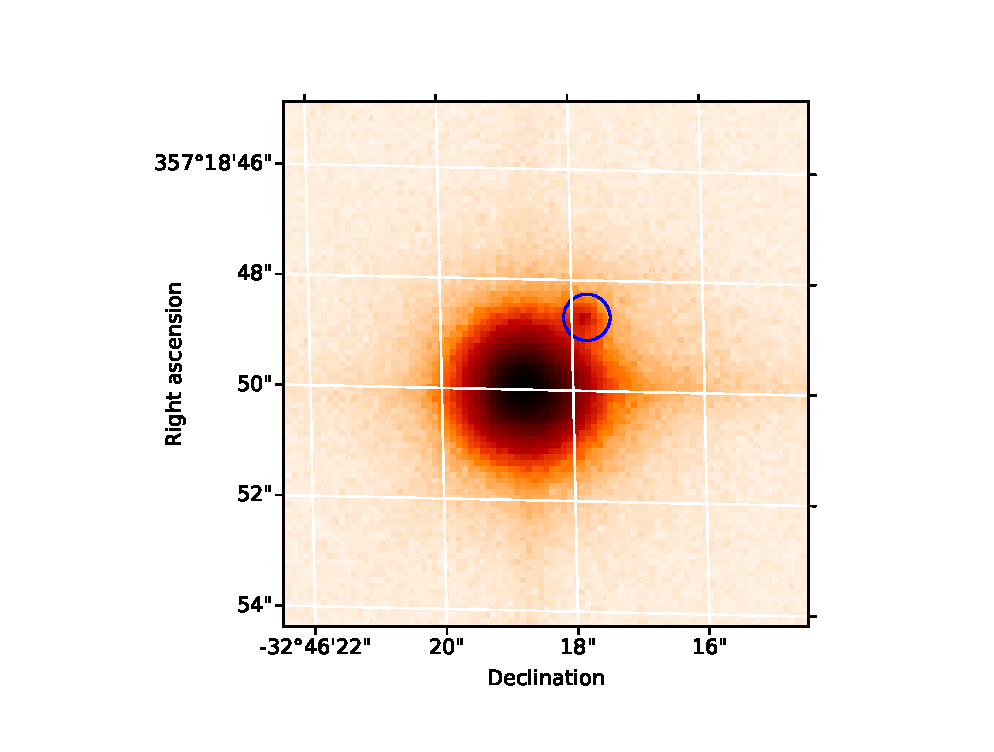
\includegraphics[]{8-Results/J2349-32/lucky.eps}
  \caption{Lucky imaging of J2349$-$32 (red arm) revealing a close companion 1.3" (blue circle) away at a position angle of $308.6 \pm 0.6^\circ$ (blue circle).}
  \label{fig:J2349-32:lucky}
\end{figure}


\begin{figure}[htb]
  \centering
  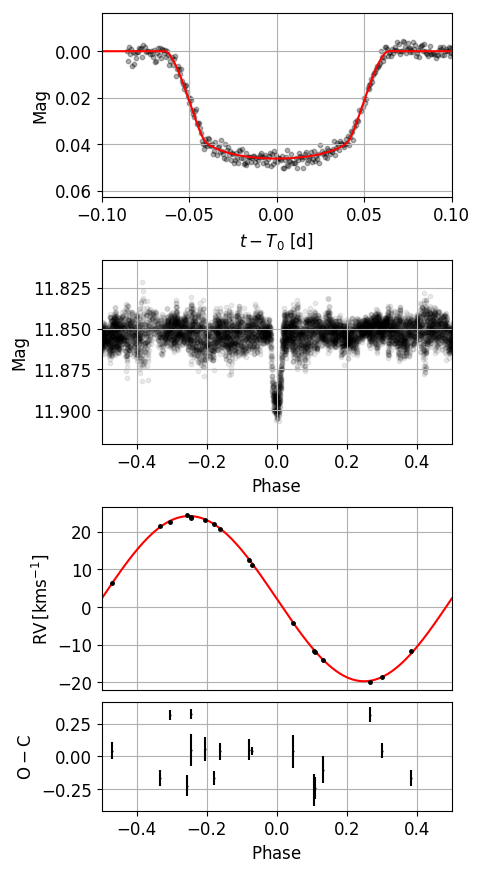
\includegraphics[scale=0.8]{8-Results/J2349-32/orbital.png}
  \caption{Orbital fit of EBLM J2349$-$32. (top panel) The detrended I-band light-curve from the SAAO 1-m telescope (black) with the best fitting transit model (red). (upper-middle panel) The phase-folded WASP lightcurve (black).  (lower-middle panel) Drift-corrected radial velocity measurements (black) with the best model (red). (bottom panel) The residuals from radial velocity model measurements.}
  \label{fig:J2349-32:orbit}
\end{figure}

J2349$-$32 was observed over three consecutive years by the WASP project. In each season I found quasi-periodic signals at periods of $4.42\, \rm d$, $4.35\, \rm d$ and $4.42\, \rm d$ with amplitudes between 3--4\,mmag. Each of these signals has a false-alarm probability $<10^{-5}$ and so I assumed this is detection of the rotational period of the primary star ($P_{\rm rot} = 4.40 \pm 0.03$\,d). From the WASP photometry, I measured $\Delta t_{\rm tr} = 0.126$\,d and $\Delta m = 0.043$ mag. corresponding to $R_\star / a \approx 0.11 $ and $k \approx 0.21$.

The best SED fit ($\chi_{\rm red}^2 = 1.24$) corresponds to a star with spectral type F7 with a low reddening ($\rm E(B \rm- \rm V) \leq 0.034$ to 1-$\sigma$). This system was included in Gaia DR2 (source ID 2314099177602409856). The $G$  magnitude was measured to be $11.413$ and the parallax is $3.43\pm 0.52\, \rm mas$ ($260 \pm 3$\,pc).  Gaia DR2 shows a single star ($G = 15.219$) 48" away at a position angle of $111^\circ$ (source ID 2314099173307737088). This source is not included in the sky annulus of the SAAO 1-m photometry, but falls within the WASP aperture where it will contribute around 3\% of the total flux. The proper motions of this star and J2349$-$32 are significantly different in right ascension and declination so I concluded that they are not associated.

J2349$-$32 was observed with lucky imaging on 2017-07-08 where two companion stars were detected. A close companion was found at a separation of $1.402 \pm 0.013$" and position angle of $308.6^{\circ} \pm 0.6^{\circ}$ (Fig. \ref{fig:J2349-32:lucky}). I measured the companion to be $5.55 \pm 0.08$\,magnitudes fainter in the TCI red-arm images; the companion was not sufficiently resolved in the TCI visible-arm images to obtain any reliable measurements. A second, distant companion was detected at a separation of $25.70 \pm 0.07$", position angle of $218.6 \pm 0.3^\circ$. I find that it is $9.0\pm0.3$\,magnitudes fainter with the TCI red-arm images and $8.5 \pm 0.3$\,magnitudes fainter in the visible-arm images. This is the same source identified by Gaia DR2 (source ID 2314099173307737088). If the closest companion is blended in the CORALIE and SAAO 1-m apertures, I estimate that it only contributes 0.6\,\% of the light and is too faint to significantly modify the transit light-curve. 

The 17 CORALIE spectra were combined to produce a spectrum with SNR$=40$. The analysis of this spectrum shows that the primary is a slightly metal-deficient star with a temperature consistent with the SED fit. There is a weak Li\,I line at 670.7\,nm from which I measured a lithium abundance $\log \rm A_{\rm Li}+12  = 2.4\,\pm \, 0.08$. This value was estimated by synthesising a small region around this line in \textsc{ispec} using fixed atmospheric parameters from wavelet analysis (Table \ref{EBLMs_atmos}) and manually adjusting the lithium abundance to obtain the best fit by-eye.


The RVs were fitted simultaneously with a single transit in I-band from the SAAO 1-m telescope to obtain the best fitting orbital solution ($\chi_{\rm red}^2 = 0.93$; Fig. \ref{fig:J2349-32:orbit}). The PPD for eccentricity is consistent with a circular orbit ($e \leq 0.05$ to $5$-$\sigma$). I find a negligible drift in systematic velocity ($\leq$ 15\,m\,s$^{-1}$\,yr$^{-1}$ to $1$-$\sigma$). The best-fitting limb-darkening temperature agrees with effective temperatures measured with SED fitting and wavelet analysis to better than $1$-$\sigma$.

% read https://arxiv.org/pdf/1404.7156.pdf

\textsc{eblmmass} predicts a primary star which has a mass and radius similar to the Sun, but is approximately 350\,K hotter. This is partly due to this being a metal-poor star, but also because it is approximately half the age of the Sun. The youthfulness of this star in conjunction with a convection zone which is unable to transport lithium to the core where it would be burnt may explain why lithium is detected with spectroscopy. The secondary component appears to be an M-dwarf below the fully convective limit.  %The M-dwarf component of J2349$-$32 sits above the 2\,Gyr isochrone ([M/H]=0 dex, where I assumed [Fe/H]$=$[M/H])  by $\approx 2\%$. I interpolate the 2\,Gyr [M/H]$ = 0.0$\, dex and [M/H]$ = -0.5$\, dex isochrones to account for [Fe/H] = $-0.28$\,dex to find a model-predicted radii of 0.192\,R$_\odot$ suggesting an inflation of 5\%.





\section{J2308$-$46}

\begin{figure}[htb]

  \centering
  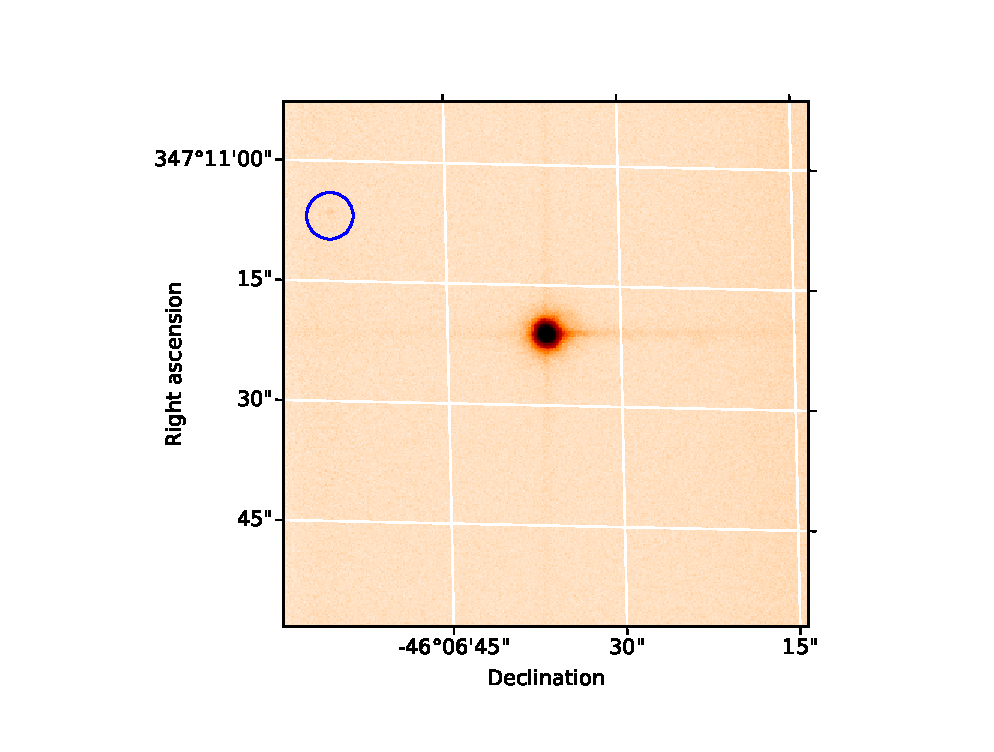
\includegraphics[]{8-Results/J2308-46/lucky.eps}
  \caption{Lucky imaging of J2308$-$46 (red arm) revealing a companion 20" away with a position angle of 208$^\circ$ (blue circle).}
  \label{fig:J2308-46:lucky}
\end{figure}

\begin{figure}[htb]
  \centering
  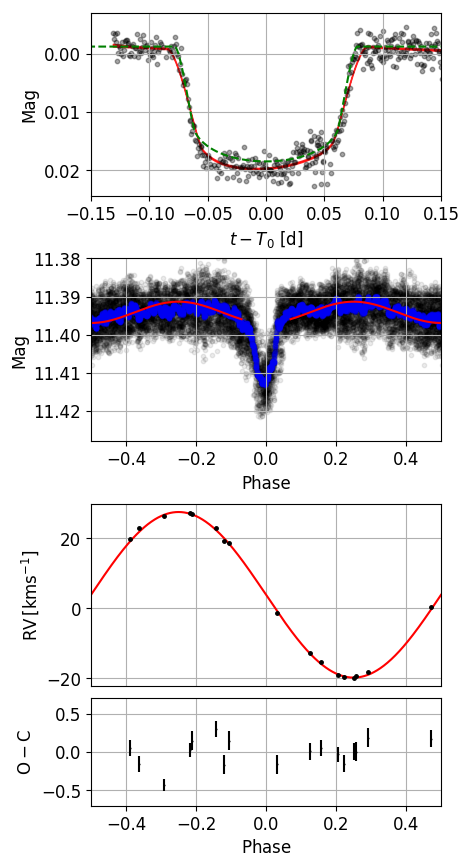
\includegraphics[scale=0.8]{8-Results/J2308-46/orbital.png}
  \caption{Orbital fit of EBLM J2308$-$46. (upper panel) R-band transit obtained from the SAAO 1-m telescope (black) with the best fitting transit model (green dashed). I also plot the best fitting transit model generated using Gaussian processes (red). (middle panel) Phase-folded WASP observations (black) and observations binned into groups of 50 (blue). I also plot the Roche model of used to approximate the out-of-transit photometry used to measure transit parameters from WASP photometry (red).  (lower panel) Drift-corrected radial velocity measurements (black) with the best fitting model (red) and residuals from the best fitting orbital model.}
  \label{fig:J2308-46:orbit}
\end{figure}


\begin{figure}[htb]
    \centering
    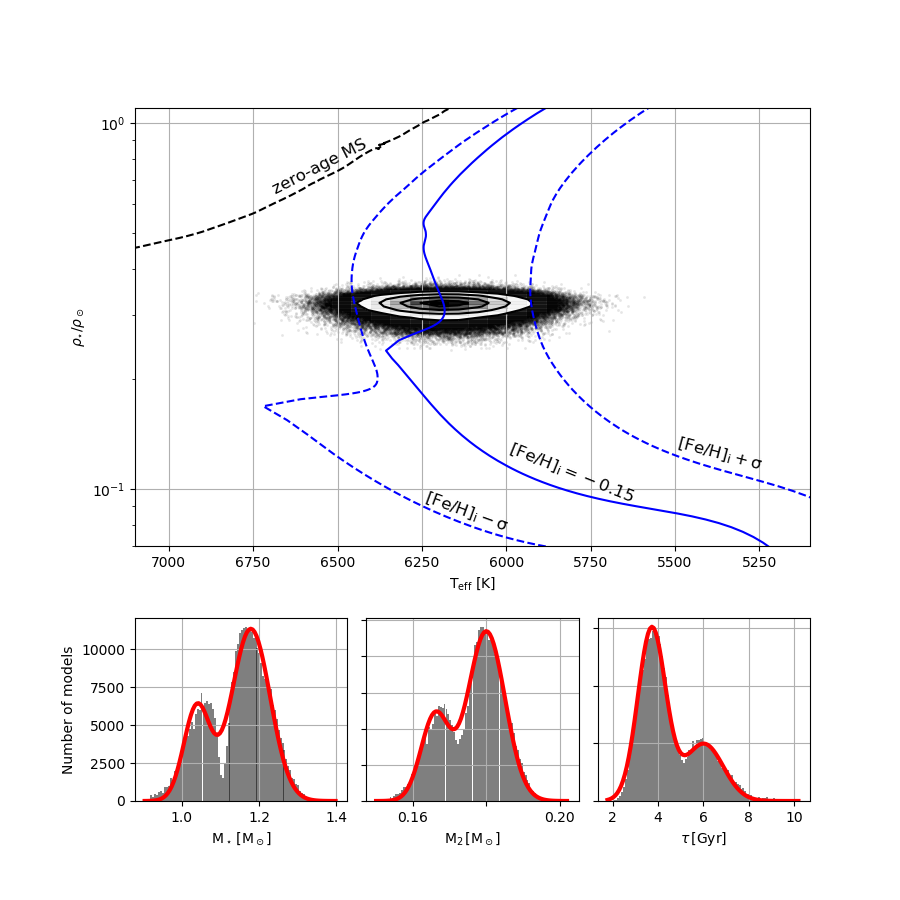
\includegraphics[scale=0.7]{8-Results/J2308-46/HR.png}
    \caption{The PPD for the density and temperature of the primary star in J2308$-$46 is shown in the top panel. The zero-age main sequence is show(black-dashed) along with the best fitting isochrone (blue-solid) and the respective isochrones for $\pm 1$-$\sigma$ in [Fe/H]. The lower panels show the PPD distributions for $M_1$, $M_2$ and $\tau$ with best-fitting double-Gaussian models in red. }
    \label{fig:J2308-46:HR}
\end{figure}

J2308$-$46 has WASP photometry spanning 5 years. The last season of data had less than 400 data points so was excluded. I measured a strong $P/2$ signal in two seasons of data. Phase folding the WASP photometry at this period reveals a moderate ellipsoidal variation with an amplitude of 5\,mmag (Fig. \ref{fig:J2308-46:orbit}). I fixed parameters associated with ellipsoidal variation to produce a good out-of-transit fit to the WASP photometry ($q = M_{2}/M_{\star}=0.05$, gravity darkening coefficient = 0.1) to estimate $\Delta t_{\rm tr} = 0.109$\,d and $\Delta m = 0.018$\,magnitudes corresponding to $R_\star / a \approx 0.20$ and $k\approx0.13$.

SED fitting measured the effective temperature of the primary star to be consistent with a spectral type F7 ($T_{\rm eff} = 6270 \pm 140$\,K; $\chi_{\rm red} = 0.77$) with a low reddening ($E(B-V) \leq 0.054$ to 1-$\sigma$). This system is included in the Gaia DR2 catalogue (Source ID 6539811294185397120; $G = 11.361$) with a parallax of $2.27 \pm 0.08$\,mas ($440.78 \pm  15.19$\,pc). There is a close companion  22.5" from J2308$-$46 at a position angle of $282^\circ$ ($G=15.388$; source ID 6539811500344886016). This is clearly resolved in the follow-up 1-m R-band photometry from SAAO and does not contaminate the sky annulus. It does fall within the WASP annulus, contributing approximately 3\% of the total flux. There is another source 48" away from J2308$-$46 at a position angle of $23^\circ$. This is also included in Gaia DR2 ($G = 14.919$; source ID 6539817204061452544) which is on the limits of the WASP aperture and would contribute less flux than the source at position angle $282^\circ$. J2308$-$46 was observed with lucky imaging on 7 July 2017 with only a single, faint companion being found, located $21.38 \pm 0.04$" away at a position angle of $208.2\pm0.4^\circ$ (Fig. \ref{fig:J2308-46:lucky}). I measured magnitude differences of $8.2 \pm 0.3$\,magnitudes in the TCI red-arm images and $8.0\pm0.2$\,magnitudes in the TCI visible-arm images. This object is included in the Gaia DR2 catalogue with Source ID 6539811289890737408 with $G=19.538$. I compared the proper motion of J2308$-$46 
%($\Delta \alpha = 26.662$\,mas\,yr$^{-1}$, $\Delta \delta = 2.496$\,mas\,yr$^{-1}$) 
with this object
%($\Delta \alpha = 1.391$\,mas\,yr$^{-1}$, $\Delta \delta = -5.137$\,mas\,yr$^{-1}$) 
 and conclude they are not physically associated.

 I co-added 22 CORALIE spectra to produce a spectrum with SNR=$20$. Wavelet decomposition shows that the primary star is a rapidly-rotating (V$\sin i \, \approx 39 \, \rm km\,s^{-1}$) and metal poor ([Fe/H] = $-0.15$ dex). This star appears to be close to the Kraft break \citep{1967ApJ...150..551K} which separates stars with deep convective envelopes and efficient dynamos from those without. Magnetic fields from these dynamos maintain a transfer of angular momentum to stellar wind resulting in magnetic breaking.  This high rotation rate and low SNR spectra makes it difficult to measure accurate radial velocities for this star. Initial attempts to find the best orbital solution resulted in 5 radial velocity measurements which differed by up to $2$\, km\,s$^{-1}$; these were excluded as outliers.

Fitting the follow-up photometry jointly with radial velocity measurements was non-trivial as clear systematic errors remained in the SAAO 1-m light-curve after initial detrending. I obtained an orbital solution in the same framework as EBLM J2349$-$32  but found an unacceptable fit around contact point 2 and the continuum prior to contact point 1 in the SAAO 1-m light-curve (see top panel of  Fig. \ref{fig:J2308-46:orbit}). I attempted to further detrend the light-curve with airmass, CCD position and time but this did not successfully remove the problem. Instead, I decided to generate a red-noise model using Gaussian processes. I used the {\sc celerite} package to model these data using a Mat\'{e}rn-3/2 covariance function (Sect. \ref{methods:rednoise}). The parameters $\log \rho$ and $\log \sigma$ tended to a value that over-fitted the noise in the light-curve if it remained as a free parameter in the joint fit. Instead, I adjusted these values ``by-eye'' until I found an acceptable red-noise model that accounted for the data around the second contact point ($\log \rho=2$ and  $\log \sigma=2$). The parameters were then fixed at these values to find an acceptable orbital solution ($\chi_{\rm red}^2 = 1.32$; Fig. \ref{fig:J2308-46:orbit}) in the same way as J2349$-$32.

The primary star is close the the ``blue-hook'' phase of its post main-sequence evolution (Fig. \ref{fig:J2308-46:HR}). This results two peaks in the PPDs for $M_\star$ , $M_2$ and $\tau$. Both solutions could be valid and so it is a requirement to fit these systems to assess the likelihood and validity of each. 
I fitted double-Gaussian models to the PPDs of $M_\star$, $M_2$, $\tau$ and $a$ which have been sorted into 100 equal bins. I used the Levenberg-Marquardt algorithm to find the optimal model vector $\textbf{m} = (A_1, \mu_1, \sigma_1, A_2, \mu_2, \sigma_2)$ for the double Gaussian model:
%
\begin{equation}
    y = A_1e^{-\frac{(x-\mu_1)^2}{2\sigma_1^2}} + A_2e^{-\frac{(x-\mu_2)^2}{2\sigma_2^2}},
\end{equation}
%
where $x$ is the position of the bin, $y$ is the number of models in the respective bin, $\mu$ is the measurement of the model, $\sigma$ is the uncertainty associated with the model, and $A$ representing the number of models at the peak of the of the distribution. 
The resulting fit for J2308$-$46 isn't entirely satisfactory; the fitted values of $\mu$ do not entirely match up with the peaks of the PPD for $M_\star$ , $M_2$ and $\tau$. This is partly due to the PPDs being poorly described by a Gaussian. Other EBLMs (e.g. J0218$-$31) have double-peaked PPDs which are well described by Gaussian, so I decided to add additional uncertainty rather than seeking a more complex model. To account for this, I add an additional uncertainty of 2\% for $M_\star$ , $M_2$ and $\tau$ which was estimated by measuring the offset between the fitted values of $\mu$ and the peaks of the respective PPDs. Moreover, the width of each PPD ($\sigma$) is underestimated upon visual inspection leading to an additional 1\% uncertainty which was determined ``by-eye''. The total additional uncertainty for each $\sigma$ is 3\%. I assessed each solution using the ratio of likelihoods. I find that the younger solution ($\tau = 3.98 \pm 0.86$ Gyr) is preferred over the older solution ($\tau = 5.81 \pm 1.0$ Gyr) with a factor $\mathcal{L}(3.98\, \rm Gyr) / \mathcal{L}(5.81\, \rm Gyr)$ $\approx 3.18$. This is moderate evidence to favour the younger solution but far from conclusive so I report both solutions in Table \ref{EBLMV_orb}. % The older solution for $M_2$ bisects the solar and [M/H]$=-0.5$ dex isochrones at 5\,Gyrs. The younger solution has an expected radii of 0.197\,$R_{\odot}$ (interpolated from [Fe/h] = $-0.15$) requiring a deflation of 4\% to match evolutionary models.





\section{J0218$-$31}

\begin{figure}[htb]
  \centering
  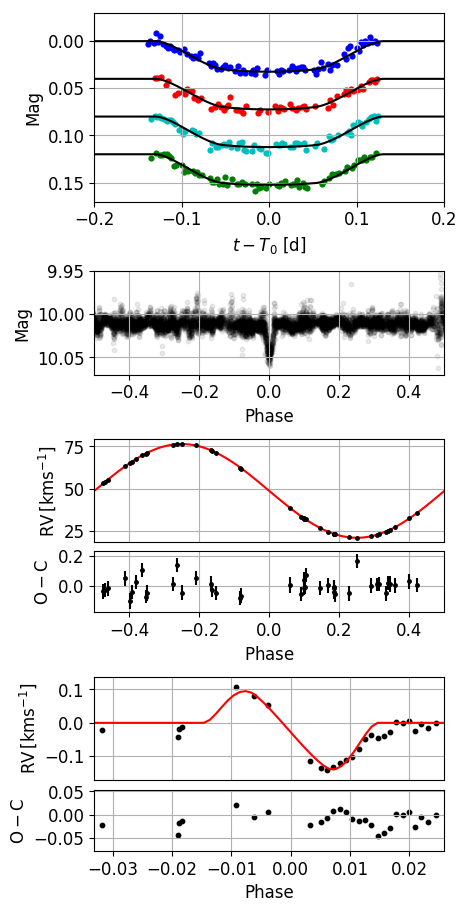
\includegraphics[scale=0.8]{8-Results/J0218-31/orbital.png}
  \caption{Orbital fit for EBLM J0218$-$31. (top panel) Transit photometry from CTIO in $g'$ (blue), $r'$ (red), $i'$ (cyan) and $z'$ (green) with best fitting models shown in black. (upper-middle panel) The phase-folded WASP lightcurve. (lower-middle panel) Drift-corrected radial velocity measurements from CORALIE with best fitting model plotted in red, along with residuals. (bottom panel) Drift-corrected radial velocity measurements during transit (the Rossiter–McLaughlin effect; black) with the best fitting model (red). Error bars have been omitted for clarity.}
  \label{fig:J0218-31:orbit}
\end{figure}


\begin{figure}
    \centering
    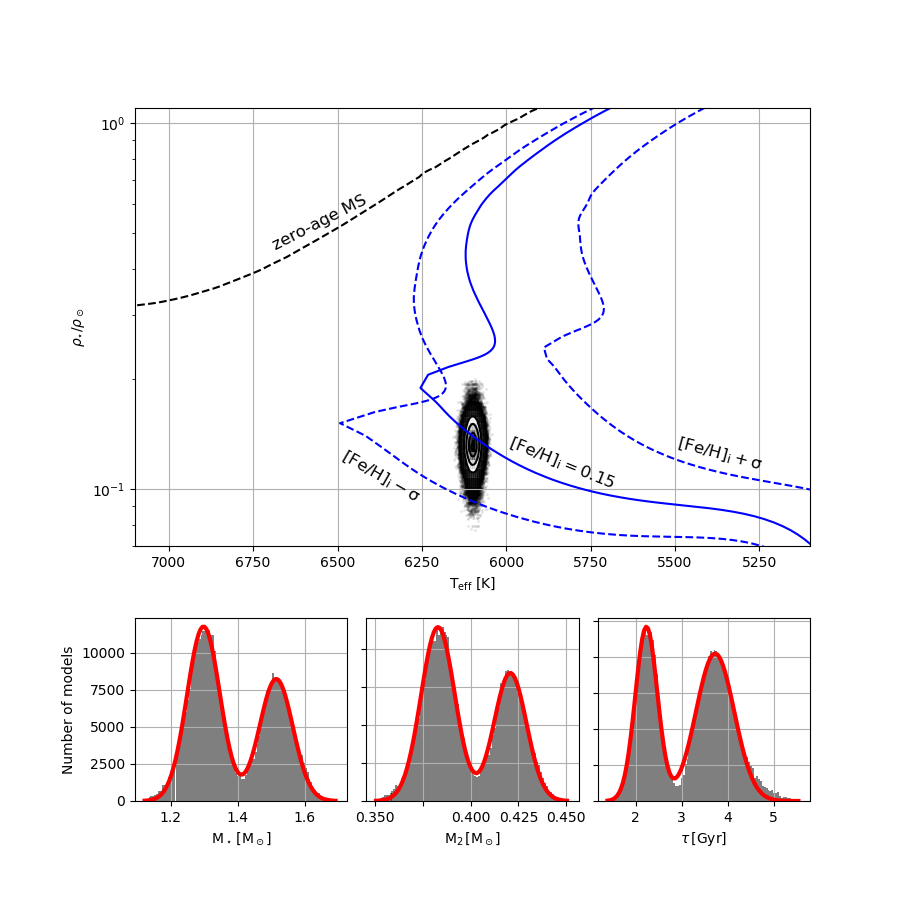
\includegraphics[scale=0.7]{8-Results/J0218-31/HR.png}
    \caption{The PPD for the density and temperature of the primary star in J0218$-$31 is shown in the top panel. The zero-age main sequence is show(black-dashed) along with the best fitting isochrone (blue-solid) and the respective isochrones for $\pm 1$-$\sigma$ in [Fe/H]. The lower panels show the PPD distributions for $M_1$, $M_2$ and $\tau$ with best-fitting double-Gaussian models in red. }
    \label{fig:my_label}
\end{figure}

J0218$-$31 was observed over three years by the WASP survey. I find a tentative detection of spot-induced variation across the three seasons ($P_{\rm rot}=2.30$\,d, $2.14$\,d and $2.60$\,d). Each have an amplitude around $1$\,mmag amongst a complex periodogram of similar (but smaller) amplitudes making it unclear whether this is due to spot-induced variations ($P_{rot} = 2.35 \pm 0.20$\,d) or poor-quality photometry. From the WASP photometry, I estimated $\Delta t_{\rm tr}= 0.241$\,d and $\Delta m = 0.03$\,magnitudes, corresponding to $R_{1}/a  \approx 0.09$ and $k \approx 0.18$.

I obtained a good SED fit ($\chi_{\rm red}^2 = 0.75$) with the effective surface temperature of the primary star consistent with a spectral type G0 ($T_{\rm eff} \approx 6020$\,K). J0218$-$31 is included in the second data release of Gaia ($G = 9.734$; Source ID 4971670729566470528) with a parallax measurement of $3.84 \pm 0.04$\,mas $ (260.13 \pm  2.85$\,pc). There are 3 close and faint companions within 22" at position angles 266$^\circ$, 332$^\circ$ and 92$^\circ$. The brightest has $G = 17.140$ ($\Delta G = 7.406$) which would contribute negligible flux to the aperture of both the WASP photometry and the follow-up R-band photometry. A brighter companion ($G = 16.015$; source ID 4971670935725243904) is located 50" away at a position angle of 330$^\circ$. This does not overlap the sky annulus of the 1-m SAAO photometry and will have a negligible flux contribution to the WASP photometry. The proper motions of these stars are not similar to J0218$-$31 and so I concluded that they are not physically associated.

I co-added fifty-three out-of-transit spectra to produce a spectrum with SNR $=30$. Using wavelet decomposition, I estimated $T_{\rm eff} = 6100 \pm 85$\,K confirming a spectral class of G0 from SED fitting. The effective temperature is 1-$\sigma$ hotter than predicted by SED fitting suggesting there could be some additional reddening that is unaccounted for. The iron content is higher than the Sun ([Fe/H] = $0.15 \pm 0.12$\,dex). There is also a strong Li\,I  line in the spectrum from which I measure a $\log A_{\rm Li}+12= 3.24 \pm 0.08$; this suggests that the convective shell of J0218$-$31 may be similar to that of J2349$-$32.

Initial attempts to determine the orbital solution resulted in a single Rossiter-McLaughlin measurement which differed from the best-fitting model by $O-C \approx 3\,\rm km\,s^{-1}$; I excluded this measurement as an outlier. I fitted the Rossiter-McLaughlin measurements alongside the out-of-transit radial velocity measurements with $g'$, $r'$, $i$ \& $z'$ band photometry to obtain the best fitting orbital solution ($\chi^2 = 1.68$; Fig. \ref{fig:J0218-31:orbit}). I initially fitted an independent value of $k$ to the $g'$, $r'$, $i$ \& $z'$ follow-up photometery. The fitted value of $k$ for each bandpass agreed with each other to 1-$\sigma$ suggesting there is no wavelength-dependent transit depths which may indicate a source of third light. However, I do find a significant drift in systematic velocity ($d(\gamma)/dt = -69.9 \pm 4.1$\,m\,s$^{-1}$yr$^{-1}$) which suggests there may be a faint third body in the system. With the addition of R-M measurements, I was able to calculate the sky-projected angle between the rotational and orbital axes, $\lambda = 4 \pm 7 ^\circ$, which is consistent with the assumption that these axes are aligned.  From this I also measured $V \sin i =  10.28 \pm 2.12\, \rm km\,s^{-1}$ which is in agreement with the value inferred from wavelet decomposition.

Similarly to J2308$-$46, J0218$-$31 has entered the ``blue-hook'' part of it's post main-sequence evolution resulting in double-peaked PPDs of $\tau$, $M_{\star}$ and $M_2$. I used the same approach for J2308$-$46 to fit a double-Gaussian to the PPDs for $\tau$, $M_{\star}$ and $M_2$ and found that the younger solution ($2.4 \pm 0.25$ Gyr, $M_{\star} = 1.55 \pm 0.05\,M_{\odot}$, $R_{\star} =  2.13 \pm 0.09\,R_{\odot}$) is favoured with almost twice the likelihood $\mathcal{L}(2.35\, \rm Gyr) / \mathcal{L}(3.80\, \rm Gyr)$ $\approx 3.55$ of the older solution. This is moderate evidence to suggest the younger solution is favoured but I report both solutions in Table \ref{EBLMV_orb} as a precaution. %Similar to J2308$-$46, the older solution of sits between the solar and and [M/H]$=-0.5$ isochrones. The younger solution requires the M-dwarf component to be deflated by a minimum of 9\% from the predicted radius of a 4\,Gyr isochrone. 








\section{J1847$+$39}

\begin{figure}[htb]
  \centering
  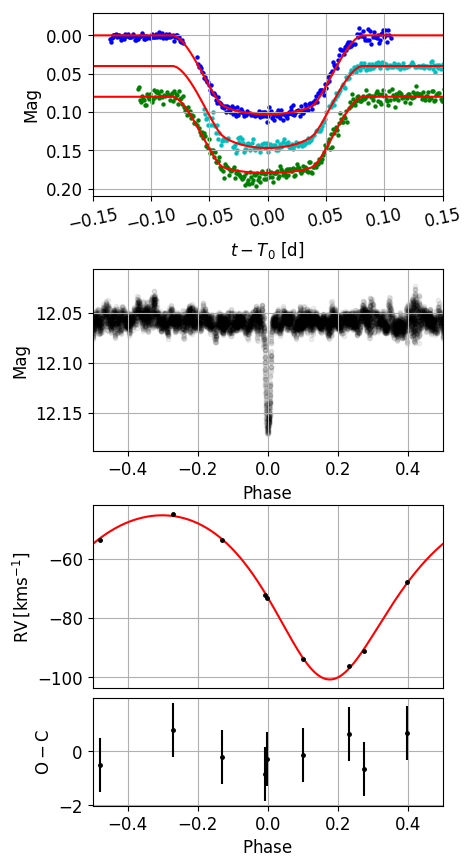
\includegraphics[scale=0.8]{8-Results/J1847+39/orbital.png}
  \caption{Orbital fit of EBLM J1847$+$39. (top panel) Single transits from the HAO in filters CBB (blue), $g'$ (cyan) and $z'$ (green) with best fitting models (red). (upper-middle panel) The phase-folded WASP lightcurve. (lower-middle panel) Drift-corrected radial velocity measurements (black) with the best fitting model (red) and residuals (lower panel).}
  \label{fig:J1847+39:orbit}
\end{figure}

J1847$+$39 was observed for three years with the WASP survey. From these three seasons, I find significant spot-induced variations at periods $7.55$\,d, $7.14$\,d and $7.17$\,d with amplitudes of  3\,--\,4\,mmag; I assumed this is a detection of rotational spot modulation at a period of $7.29\pm0.19$\,d. I find no evidence ellipsoidal variation in the WASP lightcurve from which I estimated $\Delta t_{\rm tr} = 0.02$\,d and $\Delta m = 0.10$ mag corresponding to initial estimates of $R_{\star}/a \approx 0.07$ and $k\approx0.32$.

The best SED fit estimated the primary star to be of spectral type G0 with temperature of $6020 \pm 100$\,K ($\chi_{\rm red}^2 = 1.37$). This system was included in Gaia DR2 ($G = 11.677$; source ID 2098283457595740288) with a parallax of $3.6653 \pm 0.0254$\,mas ($273 \pm 2$\,pc). The field surrounding J1847$+$39 is relatively more crowded compared to the other targets, with over 7 targets brighter than $G=17$ within 1.5'. The closest companion is 12" away ($G=17.694$; source ID 2098283457595821440) at a position angle of $196^\circ$. A magnitude difference of $\Delta G = 6.17$ results in less than 0.3\% flux contribution if it was included in the apertures of the HAO photometry. There are two bright companions 1.28' and 1.07' away at position angles of $48^\circ$ ($G = 11.577$) and $54^\circ$ ($G=12.135$) respectively. These are beyond the sky annulus of WASP but may still contribute a small amount to the total flux. The proper motions of these objects are dissimilar to J1847$+$39 and so I conclude that they are not associated.


 
Ten INT spectra were co-added to produce a spectrum with SNR$ = 30$. I used the spectral synthesis method on the wings of the  H$\alpha$ line to estimate $T_{\rm eff} = 6200 \pm 100$\,K (spectral type F8) which is consistent with the SED fit. I was able to fit 11 un-blended Fe\,I lines in the region around H$\alpha$ from which I measured [Fe/H] for each line. I took the mean of value of [Fe/H] as the iron abundance measurement with the standard deviation as the uncertainty ([Fe/H] = $-0.25 \pm 0.21\, \rm dex$). I was unable to determine $\log g$ due to the limited wavelength coverage of H1800V grating so I assumed $\log g = 4.44$ for the aforementioned synthesis and interpolation of limb-darkening coefficients.

Radial velocity measurements were fitted simultaneously with single transits in $CBB$, $g^{'}$ and $z^{'}$ filters to obtain the best fitting orbital solution (reduced $\chi^2 = 1.77$; Fig. \ref{fig:J1847+39:orbit}). J1847$+$39 has the most eccentric orbit of the sample ($e = 0.209 \pm 0.014$). I attempted to fit an independent value of $k$ for photometry in each filter and found them all to agree within $1$-$\sigma$ suggesting there is no significant third-light contamination. However, I do measure $d(\gamma)/dt = -71.9 \pm 21.7$\,km\,s$^{-1}$yr$^{-1}$ suggesting that there may be a faint third-body in the system. The best-fitting limb-darkening temperature, $T_{\rm eff,ld}$, is $\sim 600$\,K hotter than spectroscopic and photometric analysis; the reason for this is unclear.

The best fitting solution from \textsc{eblmmass} describes a star similar to the Sun in mass and size, but a fifth of it's age ($\tau = 1.10 \pm 1.80$\,Gyr). The systems eccentricity may be primordial in origin as there would have been insufficient for tidal interaction to circularise the orbit.  The M-dwarf's mass is in the convective transition ($\sim 0.35\,M_\odot$) and provides an interesting test for low-mass stellar models in a region that is highly debated. %places it within the interesting region whereby the interior transitions from partly convective to fully convective. Despite the systems youth, I find the radius of the M-dwarf to be slightly deflated with respect to evolutionary models by $\sim1$-$\sigma$.









\section{J1436$-$13}

\begin{figure}[htb]
  \centering
  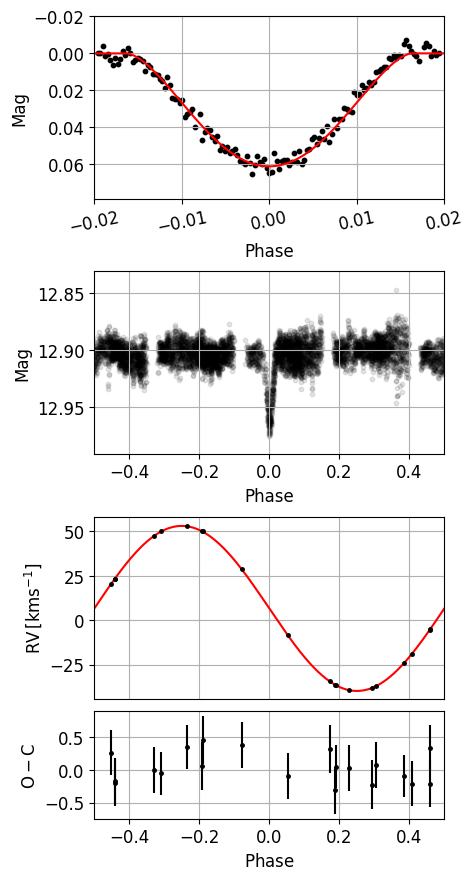
\includegraphics[scale=0.8]{8-Results/J1436-13/J1436-13_paper_plot.png}
  \caption{Orbital fit of EBLM J1436$-$13. (top panel) A single transit obtained from SAAO in R filter (black) and the best fitting transit model (red). (upper-middle panel) The phase-folded WASP lightcurve. (lower-middle panel) Drift-corrected radial velocity measurements (black) with best fitting model (red) along with residuals (lower panel). }
  \label{fig:1436-13:orbit}
\end{figure}

J1436$-$13 was observed over 3 consecutive seasons with the WASP survey. I found significant variability for each season at periods of $3.99$\,\rm d, $3.98$\,\rm d and $4.02$\,\rm d with amplitudes between 4\,--5\,$\rm mmag$. I assumed this is due to spot modulation corresponding to a rotational period $P_{\rm rot} = 4.00\pm 0.02$\,d. I find no evidence of ellipsoidal variation in the WASP photometry from which I measured $\Delta t_{\rm tr} = 0.188$\,d and $\Delta m = 0.065$\,magnitudes corresponding to initial estimates of $R_{\star}/a \approx 0.148$ and $k \approx 0.256$.

The SED fitting measured the primary star to have a spectral type of G0 ($T_{\rm eff} = 6080 \pm 355\,K$; $\chi_{\rm red} = 0.87$) with little reddining ($E(B-V) \leq 0.055$ to $1$-$\sigma$). This system is included in Gaia DR2 ($G=12.334$; source I.D 6323183619200685824) with a parallax of $2.1447 \pm 0.0513$\,mas ($466 \pm 11$\,pc). There is a faint ($G=18.994$) background star included in Gaia DR2 that is 17" away at a position angle of 302$^\circ$. This is included in the WASP aperture but contributes less that 0.1\% of the total flux.

Thirteen CORALIE spectra were co-added to produce a spectrum with SNR=$30$. Wavelet decomposition measured a value of $T_{\rm eff}$ that is around $300$\,K hotter than predicted by SED fitting suggesting that there may be some unaccounted reddening. The iron content is slightly less than the Sun ([Fe/H]$ = -0.10 \pm 0.12\, \rm dex$) and the magnesium lines are relatively narrow suggesting a low surface gravity. I was unable to identify any measurable lithium lines.

The best fitting orbital solution ($\chi_{\rm red}^2 = 1.75$) describes a transit with a high impact parameter ($b = 0.86 \pm 0.07$; Fig. \ref{fig:1436-13:orbit}). The limb-darkening temperature agrees better with SED fitting than wavelet decomposition, but is consistent with both to 1-$\sigma$. Radial velocity measurements suggest the system is circularised ($e \leq 0.004$ to $1$-$\sigma$) and there is no significant drift in systematic velocity. J1436$-$13 is slightly larger and more massive than the Sun. The uncertainty in $R_\star$ (5\%) is the largest in the sample owed to poorly constrained values of $R_\star / a$ and $k$ owed to a high impact parameter. The M-dwarf companion is the most massive of the sample ($M_2 = 0.49\,M_\odot$).




\section{J0055$-$00}


\begin{figure}
    \centering
    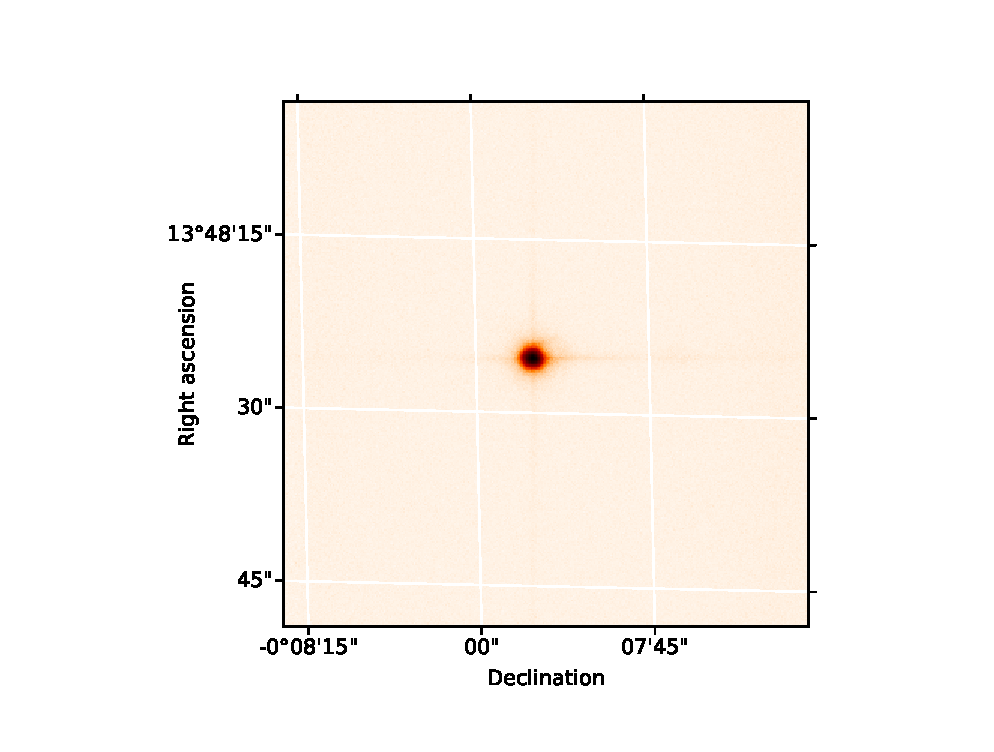
\includegraphics{8-Results/J0055-00/lucky.eps}
    \caption{Lucky imaging of J0055$-$00 (red arm) where no close companions are observed.}
    \label{fig:J0055-00:lucky}
\end{figure}

\begin{figure*}
    \centering
    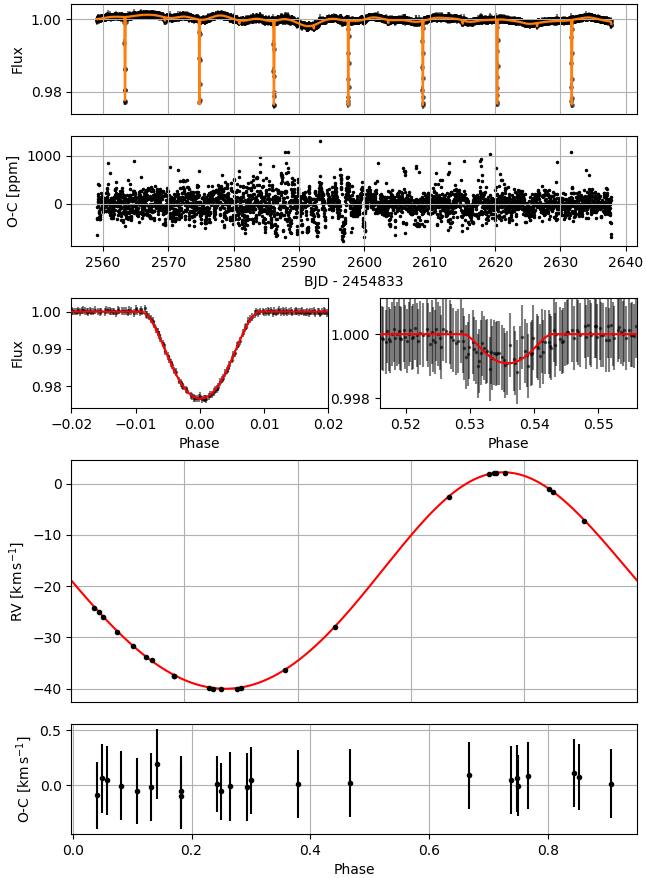
\includegraphics[scale=0.8]{8-Results/J0055-00/orbital.png}
    \caption{Orbital solution for J0055$-$00. Detrended K2 photometry (black) with model prediction using Gaussian processes (orange) is shown in the top panel with residuals in the panel below. Phase-folded K2 photometry for primary and secondary transits (black) are shown in the centre panels with best-fitting models (red).  Drift-corrected radial velocity measurements are shown (black) along with the best-fitting model (red) and residuals are shown in the lower panels.  }
    \label{fig:J0055-00:orbital}
\end{figure*}


%\iffalse
\begin{figure}
    \centering
    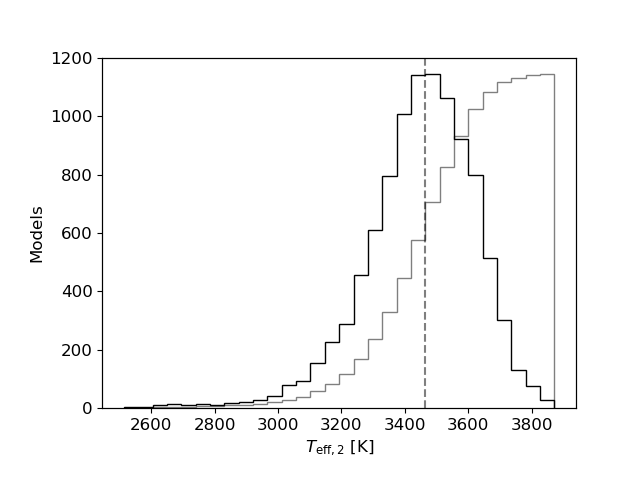
\includegraphics[scale=1]{8-Results/J0055-00/T2.png}
    \caption{Posterior probability distribution of the M-dwarf temperature for J0055$-$00. I mark the median value (dashed) along with the cumulative distribution.  }
    \label{fig:J0055-00:T2}
\end{figure}
%\fi


\begin{figure}[htb]
    \centering
    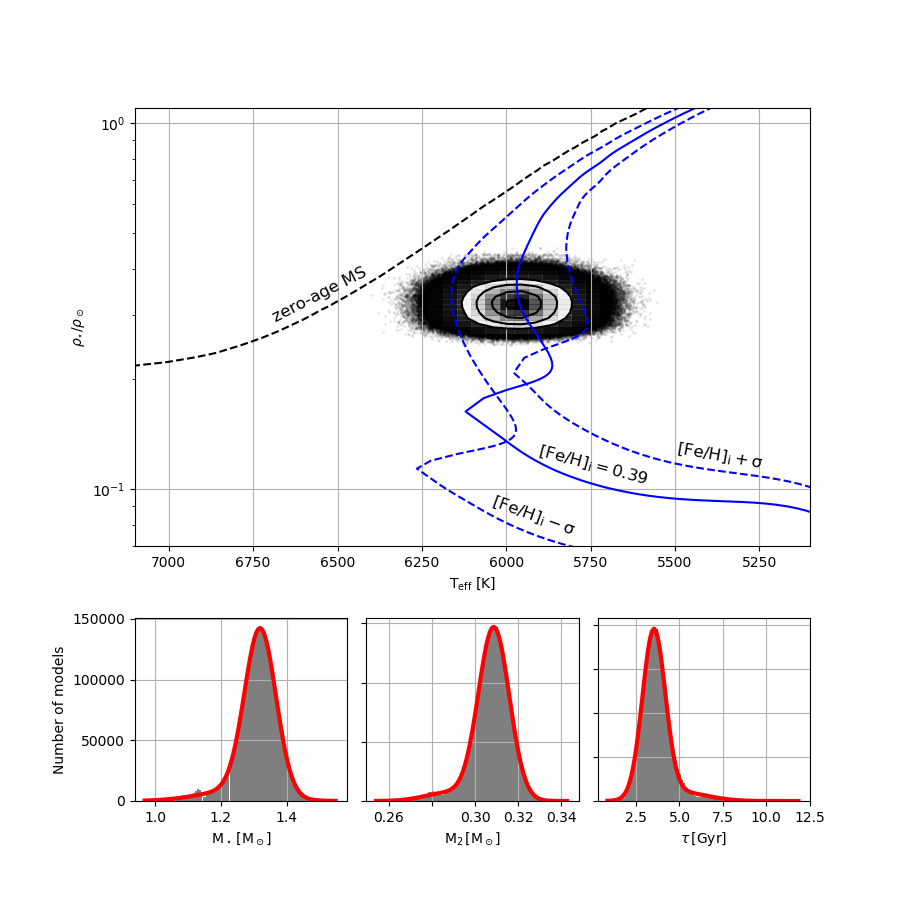
\includegraphics[scale=0.7]{8-Results/J0055-00/HR.png}
    \caption{The PPD for the density and temperature of the primary star in J0055$-$00 is shown in the top panel. The zero-age main sequence is show(black-dashed) along with the best fitting isochrone (blue-solid) and the respective isochrones for $\pm1$-$\sigma$ in [Fe/H]. The lower panels show the PPD distributions for $M_1$, $M_2$ and $\tau$ with best-fitting double-Gaussian models in red. }
    \label{fig:J0055-00:HR}
\end{figure}

% amplitude of ellipsodal
% http://www.ugastro.berkeley.edu/ay122_fall11/Presentations/SGegenheimer_TransitLightCurve.pdf

% WASP photometry
J0055$-$00 was observed over three seasons with the WASP survey. In two seasons I measured significant powers at 5.55\,d and 5.58\,d with amplitudes below 1\,mmag. Both of these periods are approximately half the orbital period, however I find no convincing evidence of ellipsoidal variation in the WASP photometry. K2 photometry appears to have variations at a similar period ($P_{\rm rot} = 5.6$\,d; 1\,mmag). 
%Using a linear limb-darkening coefficient of 0.6 and a gravity-darkening coefficient of 0.3, I estimated the predicted amplitude of ellipsoidal variation to be 0.4\,ppm. The reason this is so small is due to the large orbital separation ($a \approx 225\,R_\star$) and so the variation in the K2 photometery is most-likely caused by a spotted surface on the primary star. 
%I measured a 9.91\,d period in the third season of WASP photometry  which is likely unreliable due to the poor photometric quality. 
From the WASP photometry, I measured a primary transit transit width of 0.21\,d and depth of 0.03 magnitudes corresponding to $R_\star \approx 0.06$ and $k \approx 0.17$. There is a clear secondary eclipse visible in the K2 light curve.

% SED fit, Gaia & contamination
The SED fit is well fitted with $\chi^2_{\rm red} = 0.97$ and agrees with spectroscopy to 1-$\sigma$.
%with a moderate amount of reddening ($\rm E( \rm B \rm - \rm V) \approx 0.1$). 
There is a single star north of J0055$-$00 in Gaia DR2 that is 1.04" away at PA\,=\,359$^\circ$ ($G = 17.6986$; source ID 2536832466426328704). The difference in magnitude $\Delta G = 7$ means that it would contribute less than 0.16\% of the total flux in the WASP aperture. J2349$-$32 was observed with lucky imaging on 2017-07-19 where no other stars were detected (Fig. \ref{fig:J0055-00:lucky}). 

% Coralie spectra
Twenty-four CORALIE spectra were co-added to produce a spectrum with SNR$ = 45$. Wavelet decomposition implies a temperature consistent with a metal-rich G0-1 star. I observed a significant lithium opacity at 670.7\,nm from which I measured a $\log A_{\rm Li}  = 2.5 \pm 0.1$. J0055$-$00 has the least rotational broadening of the entire EBLM sample with a $V\sin i$ below the threshold of what can be measured with wavelet analysis ($V \sin i \leq 5\,\rm km\, \rm s^{-1}$).

% Orbital solution
The orbital solution is well fitted with a $\chi_{\rm red}^2=1.88$ (Fig. \ref{fig:J0055-00:orbital}). Similar to J0218$-$31, I measured a high impact parameter ($i = 86.80^\circ \pm 0.16^\circ$) as contact points 2 and 3 are poorly undefined. This increased the uncertainty in $k$, $R_\star / a$ and ultimately $R_1$ and $R_2$. I measured a secondary eclipse of depth  0.27\,mmag. corresponding to a surface brightness ratio $S = 0.042 \pm 0.012$. I estimate $T_{\rm eff,2} = 3464 \pm 145$\,K using \textsc{phoenix} stellar models (Fig. \ref{fig:J0055-00:T2}). Similar results have been measured for J0113$+$31 \citep{2014A&A...572A..50G} and KIC 1571511 \citep{2012MNRAS.423L...1O}. I discuss if this is expected in Sect. \ref{discuss:J0055-00T2}.

% EBLMmass
J0055$-$00 has entered the ``blue-hook`` part of its post main-sequence evolution. I observed a double-peaked PPD distribution for $M_\star$, $M_2$ and $\tau$ which was fitted in the same way as J2308$-$46 and J0218$-$31 (Fig. \ref{fig:J0055-00:HR}). The younger solution is favoured with a likelihood ratio of $\mathcal{L}_{\rm 3.5 \rm Gyr} / \mathcal{L}_{\rm 7 \rm Gyr} = 2$ and over 97\% of the models reside within the 3.5\,Gyr solution. I found that $\mu$ and $\sigma$ for the older model were not well-constrained but do a good job at fitting the PPDs of  $M_1$, $M_2$ and $\tau$. I only report the $\tau=3.5$\,Gyr solution in Table \ref{EBLMVII_orb} due to the high probability of the primary star residing on the youthful edge of the blue hook. 






\section{J0457$+$14}

\begin{figure*}
    \centering
    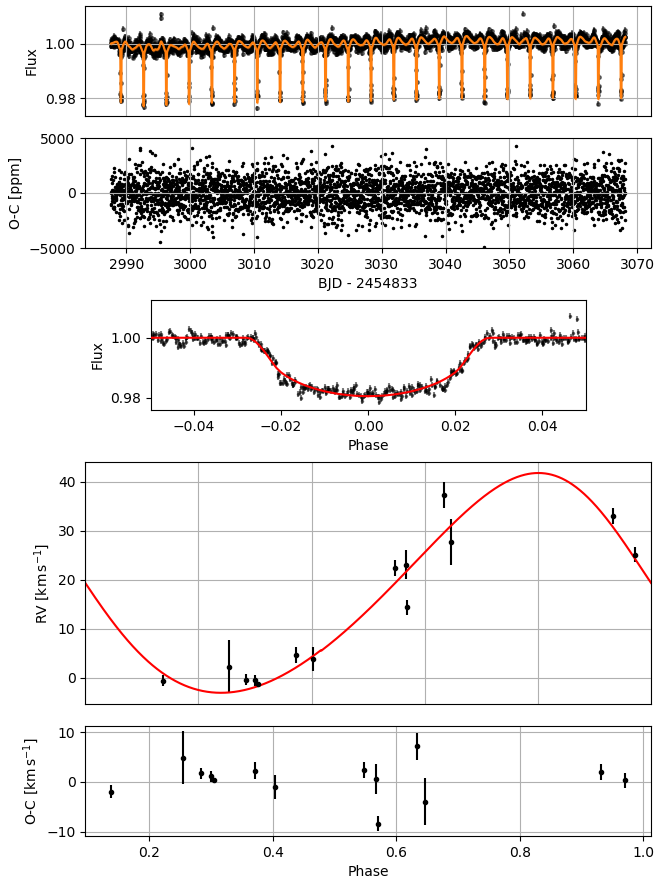
\includegraphics[scale=0.8]{8-Results/J0457+14/orbital.png}
    \caption{ Orbital solution for J0547$+$14. Detrended K2 photometry (black) with model prediction using Gaussian processes (orange) is shown in the top panel with residuals in the panel below. Phase-folded K2 photometry for the primary eclipse (black) is shown in the centre panel with the best-fitting model (red). Drift-corrected radial velocity measurements (black) and the best-fitting model (red) are shown in the lower-middle panel, along with residuals in the bottom panel.}
    \label{fig:J0457+14:orbital}
\end{figure*}

% WASP photometry
J0457$+$14 was observed over three unique seasons with WASP. The are clear peaks in the periodogram at P/2 in each season of data due to the ellipsoidal effect. Phase-folding the WASP lightcurve at these periods reveals moderate ellipsoidal variation with an amplitude $\sim 2\,\rm mmag$. This is observed in the K2 photometry with the same amplitude suggesting that the primary star is tidally deformed. Ellipsoidal variation was the dominant out-of-transit signal and I could not measure any spot-like variation. Assuming a mass-ratio of 0.6 and a gravity darkening coefficient of 0.15, I estimate the amplitude of ellipsoidal variation to be 1-3\,mmag. For the WASP photometry, I measured a transit depth of 22\,mmag and width of 0.1\,d  corresponding to $R_\star/a \approx 0.18$ and $k \approx 0.14$. 

% SED fit and Gaia
J0457$+$14 was included in Gaia DR2 ($G = 11.916 \pm 0.002$) and parallax $1.4191 \pm 0.0385$\,mas ($700 \pm 20$\,pc). There are two sources included in Gaia DR2 which are approximately $30"$ west of J0457$+$14 at position angles of 272$^\circ$ ($G = 17.243$) and 255$^\circ$ ($G = 18.002$). The proper motions of these stars from Gaia DR2 is significantly different in right ascension and declination so I concluded that they are not associated. These stars are not included in the K2 apertures and contribute less than 1\% flux in the WASP aperture. The SED fit measured the surface temperature of the primary star to be consistent with a hot, F0 star ($T_{\rm eff} \approx 7400$\,K; $\chi^2_{\rm red} = 0.96$). There is also a moderate amount of reddening fitted ($E(B-V) \approx 0.33$) consistent with the reddening inferred from the maps by \citet{2011ApJ...737..103S}.

% CORALIE spectroscopy
Fifteen spectra were co-added onto a common wavelength range to produce a spectrum of SNR$ = 30$. The precision of $T_{\rm eff}$/[Fe/H] is low because there are few lines and the quality of the individual spectra is low. The co-added spectrum has strong H$\alpha$ and H$\beta$ absorption with heavily blended weak-line absorption corresponding to a $V\sin i \approx 72 \pm 1\, \rm km\,\rm s^{-1}$. I measured a strong interstellar Na\,D line with an equivalent width $\approx 0.3\,\AA$ suggesting $E(B-V) \approx 0.11$. This is lower than measured reported by \citet{2011ApJ...737..103S} but the measured temperature is consistent with SED fitting.


% Orbital solution
The high $V \sin i$ of J0457$+$14 resulted in radial velocity measurements with uncertainties exceeding 5\,$\rm km\,s^{-1}$ in some cases. The accuracy of such measurements is the limiting factor determining the uncertainty of $f(m)$ which sets the lower-limit of uncertainty in the masses of the system. I measured $K$ to a precision of 11\% corresponding to a 33\% uncertainty in $f(m)$ ($\propto K^3$). I was able to measure a significant eccentricity in the orbital solution ($\chi^2_{\rm red} = 1.56$) despite the quality of radial velocity measurements. The system is still young ($\tau \leq 1\,\rm G\, \rm yr$ to 1-$\sigma$) which suggests the eccentricity is primordial in origin and is yet to be circularised. The primary star has a thin convective shell which is less efficient at dissipating angular momentum than cooler stars with larger convective envelopes which result in longer time scales to circularise the orbit \citep{2010A&ARv..18...67T}. The M-dwarf companion may still be in the pre-main sequence part of its evolution and thus still contracting.  




\section{J1652$-$19}

\begin{figure}
    \centering
    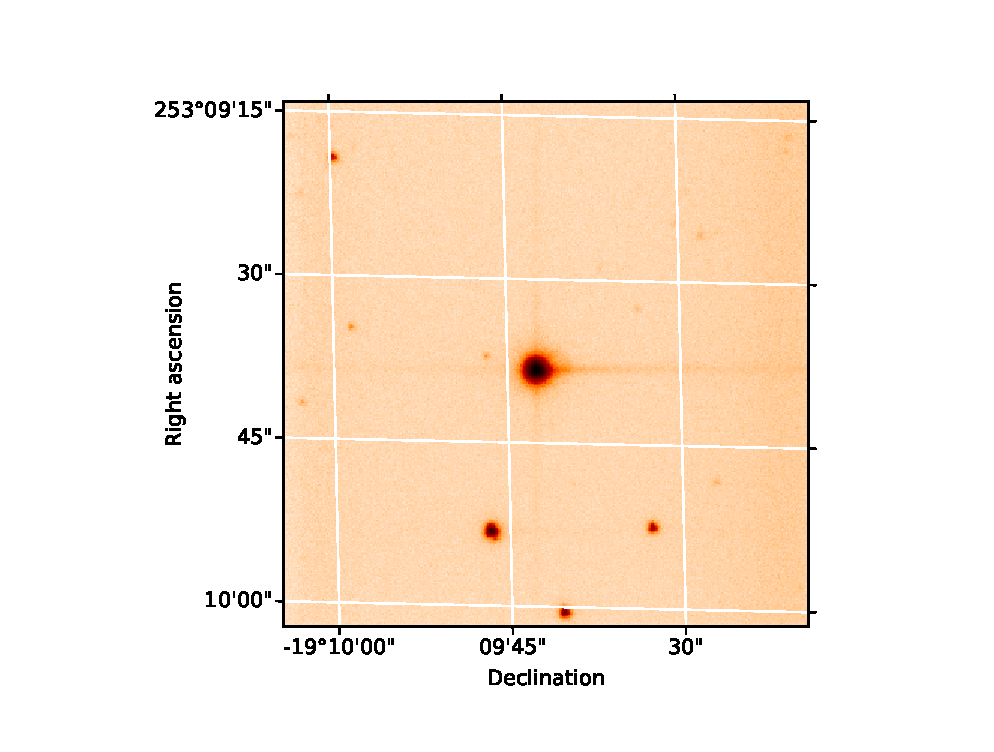
\includegraphics{8-Results/J1652-19/lucky.eps}
    \caption{Lucky imaging of J1652$-$19 (red arm).}
    \label{fig:J1652-19:lucky}
\end{figure}

\begin{figure*}
    \centering
    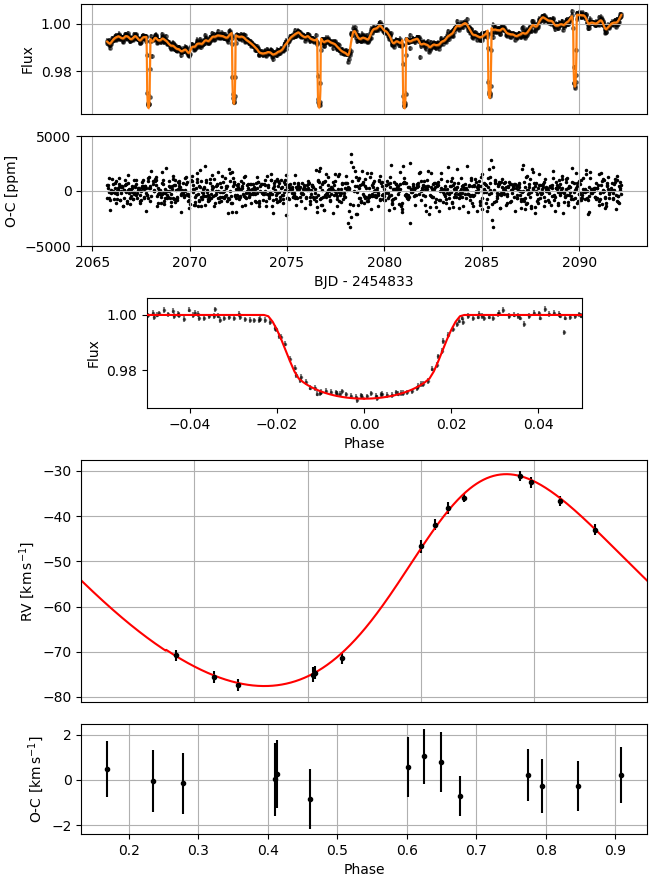
\includegraphics[scale=0.8]{8-Results/J1652-19/orbital.png}
    \caption{ Orbital solution for J1652$-$19. Detrended K2 photometry (black) with model prediction using Gaussian processes (orange) is shown in the top panel with residuals in the panel below. Phase-folded K2 photometry for the primary eclipse (black) is shown in the centre panel with the best-fitting model (red). Drift-corrected radial velocity measurements (black) and best-fitting model (red) are shown in the lower-middle panel, along with residuals in the lower panel.  }
    \label{fig:J1652-19:orbital}
\end{figure*}

% WASP photometry
J1652$-$19 was observed over 3 seasons with the WASP survey. In each season I measure a strong period between 3.7-4.3\,d (amplitudes between 4--6\,mmag) which appears to be a marginal detection of the rotational perid. The K2 photometry has a strong power peak period at 4.43\,d (amplitude of 10 mmag.) consistent with spot-induced variations. I assumed this to be a detection of the rotational period of the star ($P_{\rm rot} = 4.1 \pm 0.3$). I find no evidence of ellipsoidal variation in either WASP or K2 photometry. The transit depth in the WASP photometry is measured to be 0.03\, magnitudes deep with a duration of 0.19\,d corresponding to $R_\star \approx 0.14$ and $k \approx  0.17$.% The estimated transit depth is larger than the value of $k$ found with the joint fit.

% SED fit, Gaia & contamination
J1652$-$19 is included in Gaia DR2 (source ID: 4132067265306146560) with parallax measurements $2.081 \pm 0.113$\,mas ($481 \pm 26$\,pc). There are at least 3 other stars within 1' that are detailed in Sect. \ref{observations:K2:extract}. Lucky imaging gives a clearer picture of the field (Fig. \ref{fig:J1652-19:lucky}), where the three bright stars east of J1652$-$19 in the K2 postage stamps are clearly visible. Lucky imaging also reveals a closer and fainter companion 4.5" south of J1652$-$19 (PA = $198^\circ$). This is resolved by Gaia (source I.D. 4132067265299758720) with $\Delta G = 6.98$ and will contribute less than 0.2\% flux in the K2 aperture. The proper motion of all nearby stars from Gaia DR2 is dissimilar to J1652$-$19 and so I conclude that they are not physically associated. The best-fitting SED model ($\chi_{\rm red}^2 = 0.99$) is consistent with a primary star of spectral type F8 with a moderate amount of reddening. 

%Coralie spectra
A total of fourteen CORALIE spectra were co-added to produce a spectrum with SNR $ = 19$. Wavelet decomposition implies a temperature consistent with an F8 star that is metal rich ([Fe/H]$ = 0.18 \pm 0.06$). I identified two separate Na absorption lines (at 589.00\,nm and 589.05\,nm) corresponding to pockets interstellar Na moving at different projected velocities. I measured an EW for each Na absorption line using \textsc{ispec} and measured an independent value of reddening from the E(B-V) V. $\rm EW_{\rm Na}$ of \citet{2012MNRAS.426.1465P}: 0.14\,$\AA$ ($E(B-V) = 0.04$) and 0.11\,$\AA$ ($E(B-V) = 0.04$) for the 589.00\,nm and 589.05\,nm absorption respectively. This gives a total reddening estimate of $E(B-V) = 0.07$ and is significantly lower than the reddening estimated by \citet{2011ApJ...737..103S} despite measurements of $T_{\rm eff}$ from SED and spectral analysis agreeing within 1-$\sigma$. I was unable to measure any lithium absorbtion.

% Orbital solution
The best-fitting orbital solution is well-fitted ($\chi^2_{\rm red}$ = 1.67; Fig. \ref{fig:J1652-19:orbital}). The orbital solution describes a moderately eccentric system which has not circularised. However, the system may be pseudo-synchronised since the measured rotational period matches the orbital period. The theoretical limb-darkening coefficients from \citet{2018arXiv180407943M} did not give a good description of the shape of the transit light-curve. I decided to relax the width of the Gaussian prior for $h_1$ and $h_2$ to 0.2 and 0.45 respectively. The best fitting value of $h_1$ and $h_2$ differ from those predicted by \citet{2018arXiv180407943M} by $+0.083$ and $+0.129$ respectively. This difference exceeds what is observed for Kepler-17; an active star which displays variations on the order 0.8\% in the Kepler short-cadence lightcurves. Like Kepler-17, the amplitude of spot-induced variations in the K2 photometry is on the order of 0.81\%. The difference between expected and observed power-2 coefficients for J1652$-$19 and Kepler-17 is in the same direction for $h_1$ and opposite direction for $h_2$. The sign of the differences in $h_1$ and $h_2$ goes some way to suggest that part of the reason for this offset may be weak magnetic activity in solar-type stars that is not included in the stellar atmosphere models used to interpolate $h_1$ and $h_2$  \citet{2018arXiv180407943M}.


% EBLMMASS
The primary star has turned off the MS, but not into the ``blue-hook'' region of its  post main-sequence evolution. The system is approximately half the age of the Sun but much more massive. The primary star has likely started fusing hydrogen in a shell around the core. During this phase of stellar evolution, the effective temperature decreases and explains why I measured a $T_{\rm eff}$ similar to the primary star of J1847$+$39, despite being much more massive.



\section{J2217$-$04}

\begin{figure}
    \centering
    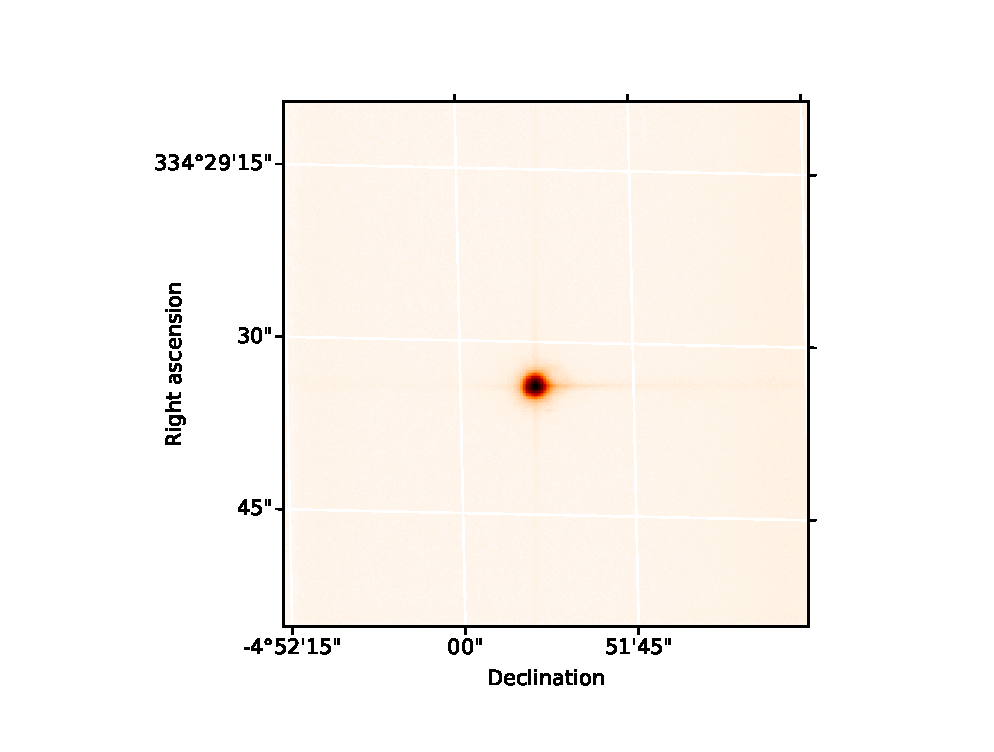
\includegraphics{8-Results/J2217-04/lucky.eps}
    \caption{Lucky imaging of J2217$-$04 (red arm) showing no significant companions nearby..}
    \label{fig:J2217-04:lucky}
\end{figure}

\begin{figure*}
    \centering
    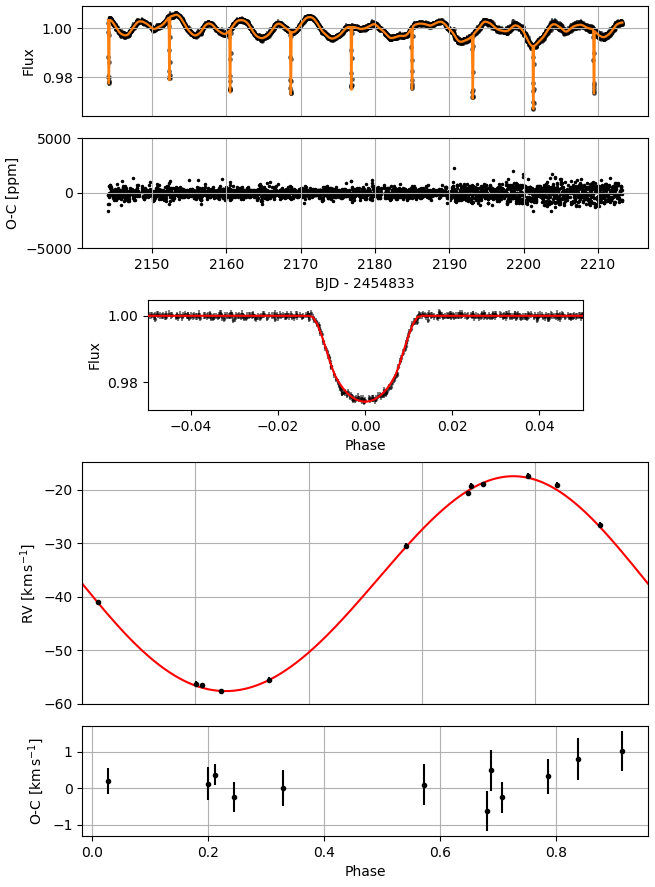
\includegraphics[scale=0.8]{8-Results/J2217-04/orbital.png}
    \caption{ Orbital solution for J2217$-$04. Detrended K2 photometry (black) with model prediction using Gaussian processes (orange) is shown in the top panel with residuals in the panel below. Phase-folded K2 photometry for the primary eclipse (black) is shown in the centre panel with the best-fitting model (red). Drift-corrected radial velocity measurements (black) and best-fitting model (red) are shown in the lower-middle panel, along with residuals in the lower panel.  }
    \label{fig:J2217-04:orbital}
\end{figure*}


\begin{figure}
    \centering
    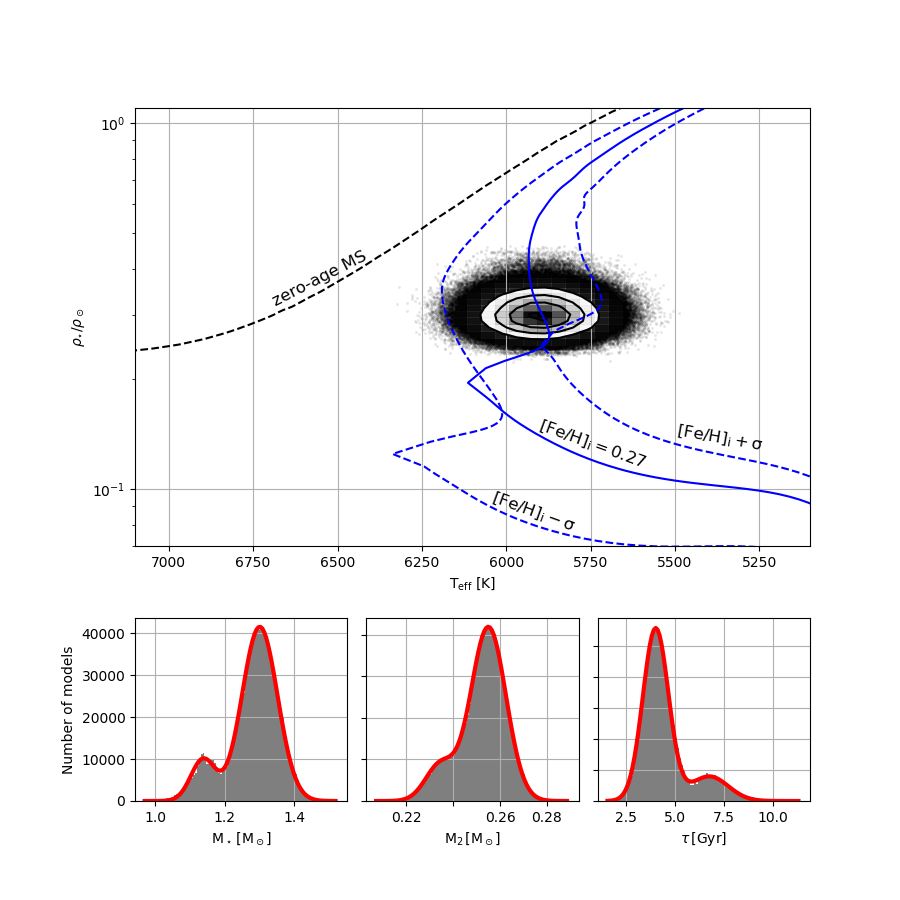
\includegraphics[scale=0.7]{8-Results/J2217-04/HR.png}
    \caption{The PPD for the density and temperature of the primary star in J2217$-$04 is shown in the top panel. The zero-age main sequence is show(black-dashed) along with the best fitting isochrone (blue-solid) and the respective isochrones for $\pm1$-$\sigma$ in [Fe/H]. The lower panels show the PPD distributions for $M_1$, $M_2$ and $\tau$ with best-fitting double-Gaussian models in red.}
    \label{fig:J2217-04:HR}
\end{figure}

% WASP photometry
J2217$-$04 was observed over two seasons with the WASP survey. I measured significant power at period 9.52\,d (3\,mmag) and 9.02\,d (5\,mmag) which is similar to the orbital period. I observed spot-like variations in the K2 photometery at a similar period and so I assumed this is a detection of stellar rotation at a period of $P_{\rm rot} = 8.16 \pm 1.58$\,d. From the WASP photometry, I measured a transit duration of 0.20\,d with depth of 0.03\,magnitudes corresponding to initial estimates $R_\star/a \approx 0.08$ and $k \approx 0.17$. 

% SED fi, Gaia & contamination
J2217$-$04 is included in Gaia DR2 (source ID: 2626910437568266240; $G = 12.003 \pm 0.001$) with parallax measurements $2.480 \pm 0.099$\,mas ($403. \pm 16$\,pc). The closest companion of J2217$-$04 is 59" away at a position angle of $85^\circ$ ($G = 15.1334\pm0.000$; source ID 2626909720308891392). This source is on the edge of the WASP aperture and would contribute 3\% of the total flux if it was included. Lucky imaging reveals no significant companions nearby (Fig. \ref{fig:J2217-04:orbital}). There is a source detected 4.5" away which is around 9 magnitudes fainter than J2217$-$04 however it is not included in Gaia DR2.  The SED fit measured a solar-like temperature consistent with a G2 spectral type ($\chi_{\rm red}^2 = 0.87$). 

% CORALIE
A total of twelve CORALIE spectra were co-added to produce a spectrum with SNR$=36$. I excluded one spectrum (BJD$= 2456150.85392$) which was incorrectly exposed. Wavelet decomposition implies the effective temperature is similar to the Sun ($T_{\rm eff} \approx 5850$\,K) with an enhanced metallicity ([Fe/H]$ = 0.27 \pm 0.06$). Wavelet analysis also implies $\log g_\star \approx 4.17$ which is corroborated by characteristically narrow Mg lines. I was unable to identify any measurable lithium absorption.  

% Orbital solution
The orbital solution is well-fitted ($\chi^2_{\rm red}$ = 1.56; Fig. \ref{fig:J2217-04:orbital}). Radial velocity measurements indicate a low eccentricity ($e\leq 0.05$ to 1-$\sigma$) resulting in a poorly constrained value of $\omega$. The impact parameter is high but the contact points are still discernible leading to robust measurements of $R_\star / a$, $i$ and $k$. The residuals of the radial velocity measurements is less than  1.1\,km\,s$^{-1}$, leading to a mass function which is constrained to 4.4\%. The measured a drift in systematic velocity consistent with zero. 

% EBLMMASS
Like many other EBLMs in this work, J2217$-$04 has evolved into the ``blue-hook'' region of its post-main sequence evolution resulting in 2 solutions for $M_\star$, $M_2$ and $\tau$ (Fig. \ref{fig:J2217-04:HR}). Fortunately, the younger solution is significantly favoured; the ratio of the likelihoods between the old young and the old solution $\mathcal{L}(3.99\, \rm Gyr) /  \mathcal{L}(6.74\, \rm Gyr) = 6.6$ with over 85\% of the models residing within the $3.99$\,Gyr solution. I report both solutions as a precaution in Table \ref{EBLMVII_orb}, marking the favoured solutions with an asterisk. 